\documentclass[11pt,a4paper]{book}

% PAQUETES POR DEFECTO:
\usepackage[utf8]{inputenc}
\usepackage[spanish]{babel}
\addto\captionsspanish{
\renewcommand{\listtablename}{Índice de tablas}
\renewcommand{\tablename}{Tabla}
\renewcommand{\lstlistlistingname}{Índice de listados de código}
\renewcommand{\lstlistingname}{Listado}
}
\usepackage{graphicx}
\usepackage{geometry}
\geometry{a4paper, margin=2.5cm} 
% --- COMANDO PERSONALIZADO PARA LÍNEAS EN BLANCO ---
% Crea una línea subrayada de la longitud especificada
% Uso: \blankline{longitud}, ej. \blankline{5cm}
\newcommand{\blankline}[1]{\underline{\hspace{#1}}}

% PAQUETES ESPECÍFICOS:
\usepackage{float}
\usepackage{longtable}
\usepackage{caption} 
\usepackage{booktabs}
\usepackage{algorithm}
\usepackage{algorithmic}
\usepackage{listings}
\usepackage{xcolor}
\usepackage[colorlinks=true, allcolors=blue]{hyperref}
\usepackage{tabularx}
\usepackage{array}
\usepackage{textcomp}
\usepackage{eurosym}

% JOSE L.
\setlength{\parindent}{0pt}
\setlength{\parskip}{6pt plus 2pt minus 2pt}
\usepackage[automake, acronym, toc]{glossaries}
\renewcommand*{\acronymname}{Lista de Acrónimos}
\glsdisablehyper
\makeglossaries
\loadglsentries{acronyms}

%\title{Simulación y optimización de la demanda energética en hogares inteligentes. Un caso de estudio con tarifas dinámicas}

%\author{}
%\date{Enero 2025}

\begin{document}

\frontmatter
% VAMOS CON LA PÁGINA DE TÍTULO
\begin{titlepage}
\centering

\vspace*{1.75cm}

\rule{12cm}{1pt}

{\Large \textbf{Título en español} \par}
{\Large \textbf{Title in English} \par} 

\rule{12cm}{1pt}

\vspace{0.75cm}

\includegraphics[width=4.25cm]{core/logo_ucm.png}
\vspace{0.75cm}

{\Large \textbf{Trabajo de Fin de Máster}} \\
%{\Large \textbf{Trabajo de Fin de Grado}} \\
{\Large \textbf{Curso 2025--2026} \par}

\vspace{1cm}
\vfill

{\Large \textbf{Autor}} \\
{\large \textbf{Nombre completo del autor} \par}

\vspace{0.25cm}

{\Large \textbf{Director}} \\
{\large \textbf{Nombre completo del director} \par}

\vspace{0.25cm}

{\large \textbf{Máster en Ingeniería Informática}}\\
{\large \textbf{Facultad de Informática}}\\
{\large \textbf{Universidad Complutense de Madrid}}

\end{titlepage}

% VAMOS CON LA SEGUNDA PÁGINA DE TÍTULO
\cleardoublepage
\thispagestyle{empty}

\centering
\vspace*{1cm}

{\Huge {Título en español}} \\
{\Huge {Title in English} \par}

\vspace*{2.5cm}

{\large \textbf{Trabajo de Fin de Máster en Ingeniería Informática}} \\
{\large \textbf{Departamento de Arquitectura de Computadores y Automática} \par}

\vspace{1cm}

{\Large \textbf{Autor}} \\
{\large \textbf{Nombre completo del autor} \par}

\vspace{0.50cm}

{\Large \textbf{Director}} \\
{\large \textbf{Nombre completo del director} \par}

\vspace{0.75cm}\vfill

{\large \textbf{Convocatoria:} Junio 2025}\\
{\large \textbf{Calificación:} 10 (Matrícula de Honor)}

\vspace{1.00cm}\vfill

{\large \textbf{Máster en Ingeniería Informática}}\\
{\large \textbf{Facultad de Informática}}\\
{\large \textbf{Universidad Complutense de Madrid} \par}
{\large \textbf{21 de julio de 2025}}

























\clearpage

\chapter*{Resumen}
\addcontentsline{toc}{chapter}{Resumen}
En el contexto del sistema energético actual y la creciente penetración de fuentes renovables en la red eléctrica, la gestión eficiente se presenta como un reto para garantizar su estabilidad. Este \gls{tfm} propone una herramienta de simulación y optimización del consumo energético en hogares conectados que responde a tarifas eléctricas dinámicas. El objetivo principal es contribuir a una mayor flexibilidad en el consumo tanto residencial como no residencial, reduciendo así los picos de demanda mediante decisiones de carga informadas y automatizadas.

Se emplea el formalismo \gls{devs}, para modelar y simular el comportamiento de distintos dispositivos eléctricos. La \mbox{simulación} se complementa con un algoritmo metaheurístico de \gls{sa}, que permite optimizar los planes de carga en función de los precios de la electricidad y las restricciones definidas por el usuario.

La herramienta desarrollada en Python, incluye una interfaz gráfica intuitiva que permite a los usuarios introducir sus preferencias y visualizar los resultados del proceso de optimización. El diseño modular de la arquitectura permite su escalabilidad y adaptación a diferentes escenarios, y se ha validado mediante un conjunto de pruebas de convergencia.

Los resultados demuestran que es posible desplazar parte del consumo eléctrico hacia franjas horarias con menor coste, sin comprometer las preferencias del usuario ni requerir su intervención directa. Esto evidencia el potencial de los \gls{hems}, como instrumentos clave para la flexibilización de la demanda. A pesar de algunas limitaciones identificadas, como la simplificación del modelo de tarifas o la falta de conexión con datos en tiempo real, el sistema propuesto sienta las bases para futuros desarrollos que podrían integrar más dispositivos, múltiples hogares e incluso comunidades energéticas enteras. En conjunto, esta propuesta representa un paso significativo hacia hogares más inteligentes, y activos dentro del nuevo ecosistema energético.

\vspace{1cm}

\noindent\textbf{Palabras clave: }\textit{HEMS, IoT, DEVS, Flexibilidad eléctrica, Gestión de la demanda, Recocido simulado}

\chapter*{Abstract}
\addcontentsline{toc}{chapter}{Abstract}
In the context of today’s energy system and the increasing penetration of renewable sources in the power grid, efficient management emerges as a key challenge to ensure grid stability. This master's thesis proposes a simulation and optimisation tool for household energy consumption that responds to dynamic electricity pricing. The main objective is to promote greater flexibility in both residential and non-residential consumption, reducing demand peaks through informed and automated load management decisions.

The \gls{devs} formalism is used to model and simulate the behavior of various electrical devices. The simulation is complemented by a metaheuristic \gls{sa} algorithm, which optimizes load scheduling based on electricity prices and user-defined constraints.

The tool, developed in Python, includes an intuitive graphical user interface that allows users to input their preferences and visualise the results of the optimization process. Its modular architecture enables scalability and adaptation to different scenarios, and has been validated through a set of convergence tests.

The results show that it is possible to shift part of the energy consumption to lower-cost time periods without compromising user preferences or requiring direct intervention. This highlights the potential of \gls{hems} as key instruments for demand-side flexibility. Despite some identified limitations, such as simplified tariff modeling and lack of real-time data integration, the proposed system lays the groundwork for future developments that could incorporate more devices, multiple households, or even entire energy communities. Overall, this work represents a significant step toward smarter, more active homes within the emerging energy ecosystem.

\vspace{1cm}

\noindent\textbf{Key words: }\textit{HEMS, IoT, DEVS, Energy flexibility, Energy demand management, Simulated annealing}

\printglossaries
\tableofcontents 
\listoftables
\listoffigures
\lstlistoflistings

%Empiezan secciones
\mainmatter

%Intro
\chapter{Introducción}

% Entradilla iría aquí: explicando un poco lo que hay en este capítulo.

% Ahora te propongo una estructura para este capítulo:

%------------------------------------------
% 1. Contexto y Relevancia del Problema
%    - Desafíos Energéticos Actuales
%      - Breve descripción de la necesidad urgente de soluciones energéticas sostenibles.
%      - Mención de los objetivos globales de descarbonización y la transición energética.
%    - Impacto del Consumo Energético en Edificios y Hogares
%      - Estadísticas sobre el consumo energético en el sector residencial.
%      - Importancia de la gestión eficiente de la energía en hogares para alcanzar los objetivos de sostenibilidad.
%
% 2. Marco Normativo y Político
%    - Agenda 2030 y Objetivos de Desarrollo Sostenible (ODS)
%      - Enfoque en el ODS 11: Ciudades y comunidades sostenibles.
%      - Mención de la Ley 7/2021 de cambio climático y transición energética en España.
%    - Iniciativas Nacionales e Internacionales
%      - Breve resumen de las políticas y regulaciones que promueven el uso de energías renovables y la gestión de la demanda.
%
% 3. Desafíos Técnicos y Oportunidades
%    - Integración de Energías Renovables
%      - Descripción de los retos asociados a la variabilidad de las fuentes renovables.
%      - Necesidad de flexibilidad en la red eléctrica para gestionar la oferta y la demanda.
%    - Tecnologías Emergentes
%      - Rol del Internet de las Cosas (IoT) en la gestión energética.
%      - Importancia de los sistemas de gestión de energía doméstica (HEMS) y programas de respuesta a la demanda (DR).
%
% 4. Objetivos del Estudio
%    - Desarrollo de una Herramienta de Simulación
%      - Propuesta de una herramienta para simular la gestión del consumo eléctrico en hogares inteligentes.
%      - Enfoque en la optimización del consumo mediante tarifas dinámicas.
%    - Prototipo de Validación
%      - Diseño de un prototipo para validar la funcionalidad del sistema propuesto.
%
% 5. Metodología (de esto escribo yo un primer borrador, José Luis)
%    - Modelado y Simulación DEVS
%      - Introducción al uso de DEVS para modelar el sistema de gestión energética.
%    - Optimización de la Configuración de Carga
%      - Breve mención de los métodos de optimización considerados (algoritmos genéticos, recocido simulado, etc.).
%
% 6. Estructura del Documento
%    - Breve descripción de cómo está organizado el resto del TFM.
%------------------------------------------
Esta sección establece las bases para comprender la creciente complejidad de la gestión energética en entornos domésticos inteligentes. Se analizan el contexto actual y los desafíos tecnológicos y regulatorios, para culminar en la presentación de los objetivos, la metodología innovadora basada en simulación \gls{devs} y la hoja de ruta de este \gls{tfm}, que busca proponer soluciones eficientes ante la dinámica de las nuevas tarifas eléctricas.

\section{Contexto y relevancia del problema}

La búsqueda de soluciones energéticas sostenibles se ha vuelto en los últimos años cada vez más urgente, motivada por el desafío global de descarbonizar el modelo energético actual y la necesidad de una transformación tecnológica para adaptar las redes al nuevo contexto en el que vivimos \cite{futured2024}. Los gobiernos de todo el mundo han establecido objetivos para esta transición, con el propósito de mitigar los efectos del cambio climático y garantizar un futuro para las próximas generaciones. En respuesta a este desafío, se están desarrollando y proponiendo productos innovadores, así como cambios en la actual gestión de la red eléctrica. Este apartado tiene como objetivo profundizar en el problema, específicamente en el consumo energético de los inmuebles, ya que representa un porcentaje significativo del consumo total de energía. 

En el caso de España, durante el periodo 2020-2022, el sector edificios, tanto residenciales como no residenciales, representaba el 32\% del consumo final, del cual el 59\% corresponde a las viviendas. Aunque este dato se encuentra \mbox{ligeramente} por debajo de la media de la Unión Europea, cuyo sector residencial conforma el 25.8\% del consumo final total, este constituye una proporción significativa del uso energético nacional. Por ello, una gestión eficiente de la energía en los hogares es clave para alcanzar los objetivos de sostenibilidad \cite{estrategiaDesarrolloSostenible2022, eurostat2023buildings, odysseeSpain2024}.

\section{Marco normativo y político}

El 25 de septiembre de 2015, las Naciones Unidas, de las que España forma parte, aprobaron un conjunto de metas globales conocido como la Agenda 2030, compuesta por 17 \gls{ods}. Como parte del plan nacional de respuesta, la Ley 7/2021, de cambio climático y transición energética, establece un objetivo de reducción de emisiones de gases de efecto invernadero del 23\% respecto a niveles de 1990 para el conjunto de toda la economía \cite{objetivosReduccion2025}. 

Este proyecto se enfoca en el \gls{ods} 7, \textit{Energía asequible y no contaminante} y el 13, \textit{Acción por el clima}. Ambos buscan asegurar el acceso a recursos energéticos limpios, que se adapten a la situación climática actual \cite{agenda2030espana}. En esta línea, este \gls{tfm} explora la facilitación de la optimización de la demanda, con el objetivo de incentivar un consumo más sostenible que permita una creciente penetración de fuentes renovables y, en general, una adaptación a un modelo más flexible condicionado por el clima.

En el ámbito europeo, el Pacto Verde Europeo establece una hoja de ruta para alcanzar la neutralidad climática en 2050, promoviendo la integración de energías renovables y la eficiencia energética. En línea con estos objetivos, la Directiva de la \gls{ue} 2023/2413, que modifica y refuerza la anterior 2018/2001, eleva el objetivo vinculante de energía renovable al 42,5\% para 2030. Esta actualización impulsa el desarrollo de fuentes limpias y la reducción de la dependencia de combustibles fósiles, centrándose en la descarbonización de sectores clave.

A nivel nacional, el Plan Nacional Integrado de Energía y Clima \gls{PNIEC} 2021-2030 plantea un incremento significativo de la generación renovable, con un objetivo de al menos un 74\% de electricidad proveniente de fuentes renovables en 2030 \cite{pniec2021}. Además, el Real Decreto 244/2019 regula el autoconsumo eléctrico, permitiendo la compensación de excedentes y fomentando la participación ciudadana en la producción de energía.

Para alcanzar estos objetivos, la gestión de la demanda se impulsa a través de mecanismos como las tarifas eléctricas basadas en señales de precio horario, la flexibilización del consumo mediante el almacenamiento energético y la digitalización de la red eléctrica. Estas estrategias permiten optimizar el uso de la energía, reducir los picos de demanda y favorecer la integración de energías renovables \cite{gestionDemanda2022}.

En definitiva, el marco normativo actual busca favorecer la transición hacia un modelo energético más sostenible, promoviendo tanto el desarrollo de energías renovables como la implementación de estrategias de gestión de la demanda para mejorar la eficiencia del sistema eléctrico, sin embargo, este proceso se enfrenta a numerosos retos.

\section{Desafíos técnicos y oportunidades}

\subsection{Integración de energías renovables}
Tradicionalmente, las redes eléctricas han transmitido principalmente energía proveniente de fuentes no renovables, conocidas por su mayor previsibilidad. A diferencia de estas fuentes, la producción de energía renovable está \mbox{influenciada} por factores como las condiciones climáticas y la hora del día. Además, se está produciendo una mayor electrificación de la demanda con nuevos usos, añadiendo presión durante las horas pico \cite{cordisPredicting2023}.
Por ello, la flexibilidad del sistema eléctrico es fundamental para mantener el equilibrio entre la oferta y la demanda, así como para enfrentar la incertidumbre en sistemas eléctricos con una alta penetración de energías renovables, cuya producción está influenciada por factores externos \cite{Impram2020ChallengesOR}; \cite{Rahman2024AnOO}. Si bien en la fecha en la que se presenta este trabajo las causas del apagón sufrido en la Península Ibérica el pasado 28 de abril de este mismo año no se conocen, se ha señalado que una posible causa podría estar relacionada con fluctuaciones en la generación energética proveniente de fuentes renovables. Esto evidencia aún más la urgencia de una adaptación de nuestro consumo al contexto energético actual.

Existen numerosas maneras de trabajar la flexibilidad de una red eléctrica, no obstante, en este proyecto nos centramos en la flexibilidad del lado de la demanda, es decir, el ajuste de patrones de consumo en respuesta a señales del mercado o problemas en la red, utilizando \gls{dr} y \gls{hems}. Esto implica concentrarse en cambiar los patrones de consumo en respuesta a las señales del mercado o problemas de la red, en lugar de ajustar la generación. Este enfoque no excluye el ajuste de la generación, sino que lo complementa dentro de un sistema energético integrado y flexible. Es decir, la gestión activa de la demanda busca optimizar el uso de la generación existente, especialmente la renovable \cite{renewableRevolution2024}. Los programas \gls{dr}, benefician a las empresas distribuidoras además de a los clientes, ya que las empresas encuentran de esta manera un modo de gestionar los picos de la demanda, mientras que los usuarios reducen su gasto en energía. 

El funcionamiento de un \gls{dr} es el siguiente \cite{demandresponse2025}:
\begin{enumerate}
    \item El operador de la red identifica un posible problema de estabilidad en el sistema y envía una notificación al agregador para activar un servicio de equilibrio.
    \item El agregador recibe la notificación y aplica algoritmos especializados para optimizar la distribución de la demanda eléctrica entre los clientes de su cartera, ajustando el consumo energético según sea necesario (reducir o incrementar).
    \item Los clientes designados ajustan su nivel de consumo o generación de \mbox{energía}, ya sea de forma automática mediante sistemas inteligentes o \mbox{manualmente}.
    \item La regulación de la carga realizada por los clientes se pone a disposición del operador de la red para mantener el equilibrio.
    \item Una vez verificado que el servicio de equilibrio se ha ejecutado correctamente, el cliente recibe la compensación correspondiente, de acuerdo con los términos establecidos en el contrato.
\end{enumerate}

Dentro de este tipo de programas cabe hacer una clasificación de los diferentes subgrupos que existen. Este diagrama, adaptado del trabajo de \cite{renewableRevolution2024}, lo organiza tal como se ilustra en la Figura \ref{fig:programa-dr}.

\begin{figure}
    \centering
    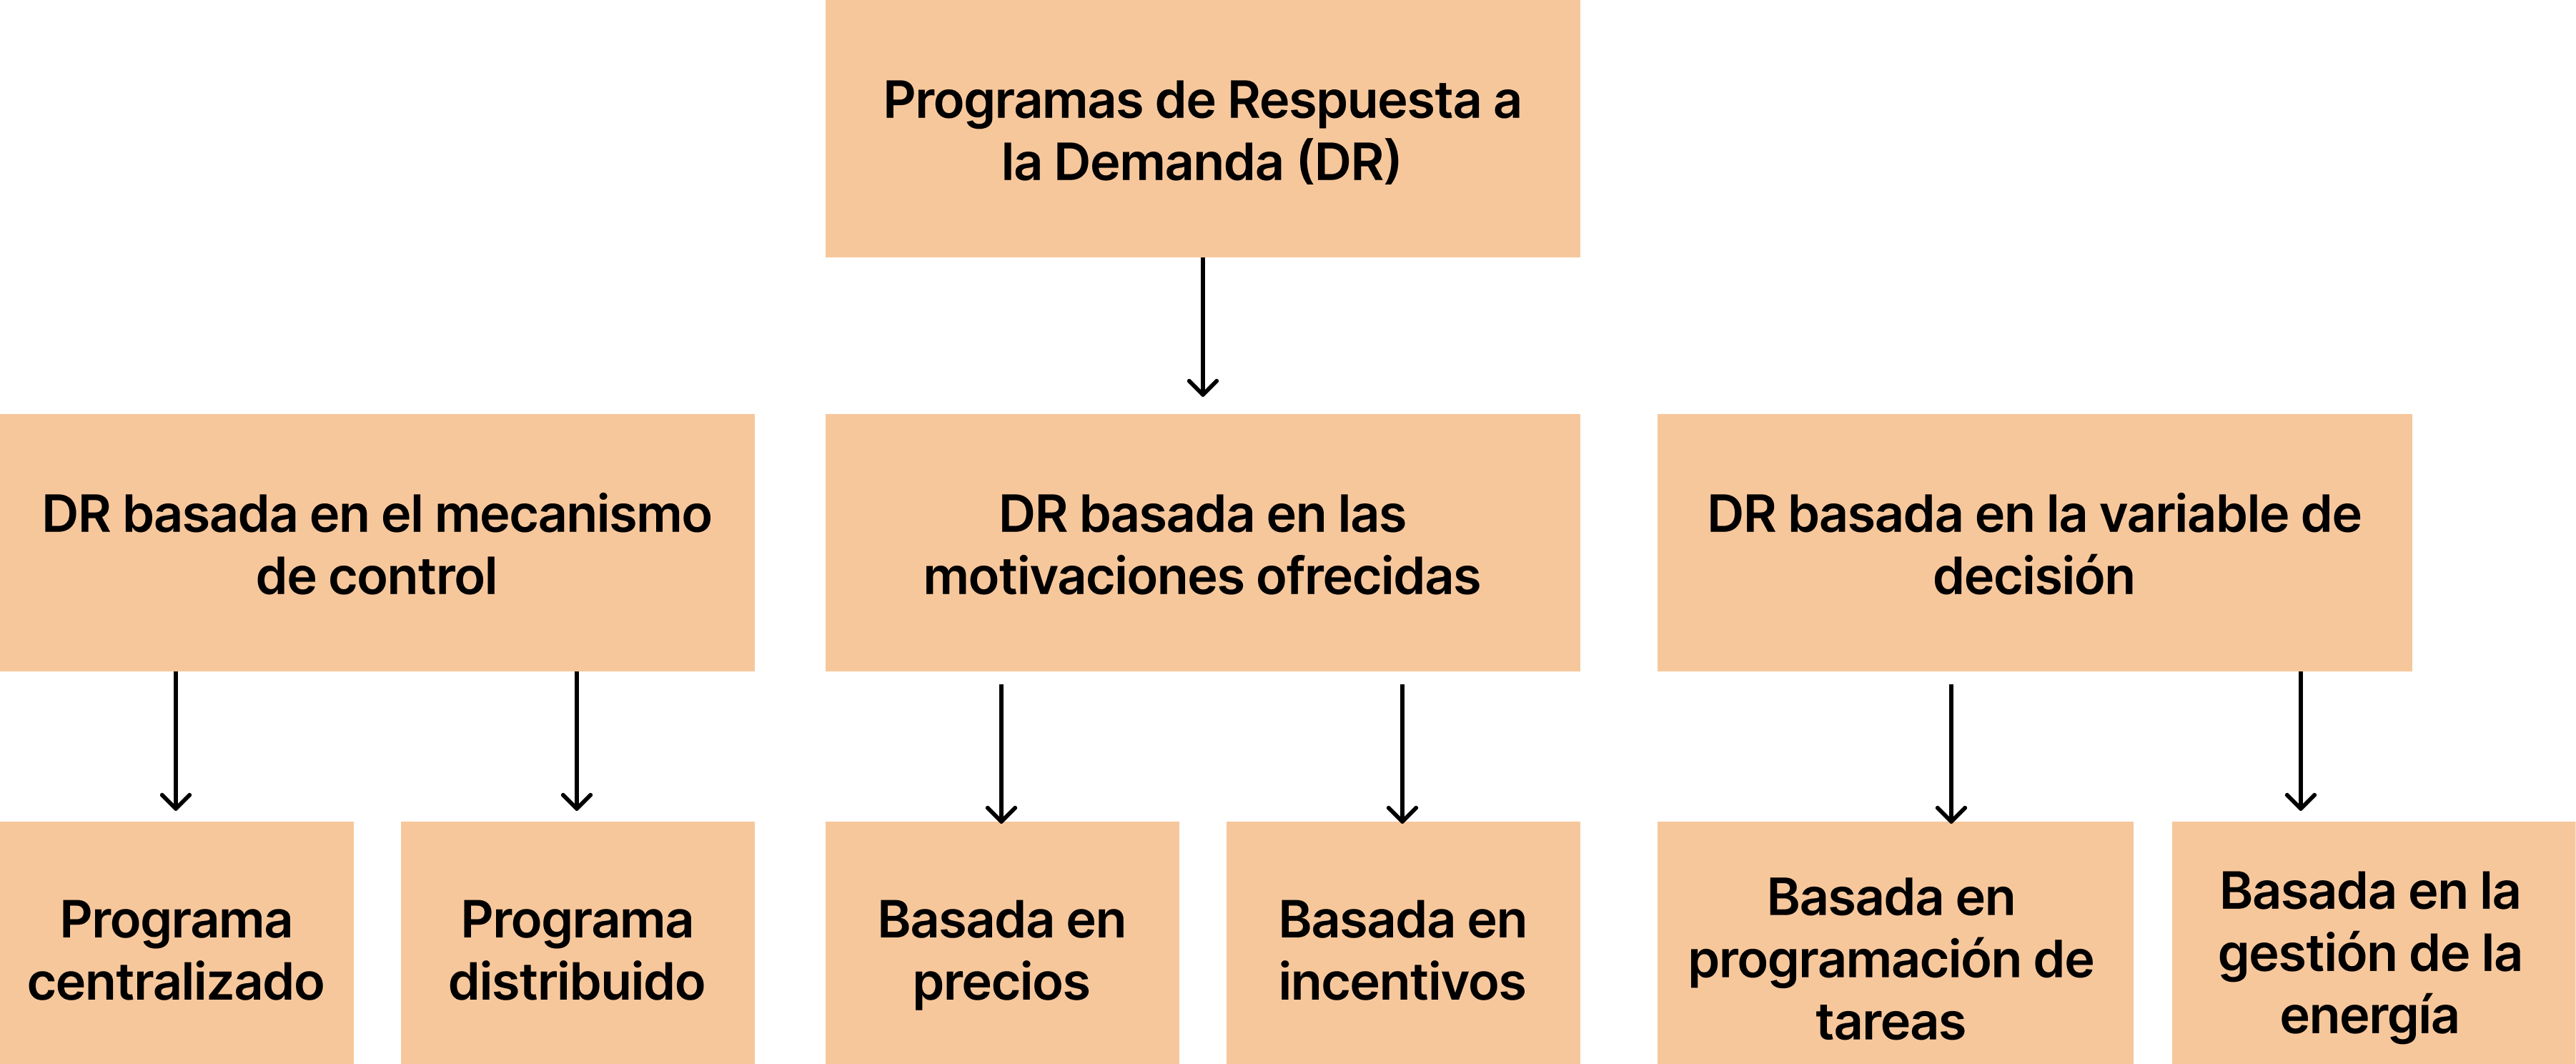
\includegraphics[width=1\linewidth]{fig/diagrama_DR.png}
    \caption{Clasificación de programas DR}
    \label{fig:programa-dr}
\end{figure}

El programa de respuesta a la demanda que se propone en este trabajo, se trata de un sistema inteligente que gestiona el consumo de los dispositivos de manera automática, sin necesidad de un papel activo por parte del usuario. También, optimiza el consumo de los dispositivos sin depender de incentivos externos o cambios manuales. Por lo tanto, según esta clasificación, se trata de un DR basada en la gestión de la energía.


\subsection{Tecnologías emergentes}
El \gls{iot}, se refiere a una red de dispositivos físicos, vehículos, electrodomésticos y otros objetos físicos que están integrados con sensores, software y conectividad de red que les permite recopilar y compartir datos \cite{IBMIoT2025}. Por ello, el \gls{iot}  tiene un rol clave en la gestión de la energía en los hogares, facilitando la interacción entre los consumidores y los proveedores de energía, y permitiendo una gestión más inteligente del consumo energético en los hogares \cite{ioT2023}. Generalmente, una solución \gls{iot} esta compuesta por los elementos que se muestran en la Tabla \ref{tab:componentes_iot} \cite{dominguez2022overview}.

\renewcommand{\arraystretch}{1.2} % Ajuste de espacio entre filas
\begin{longtable}{|p{4cm}|p{8cm}|}
    \caption{Componentes de una solución IoT} \label{tab:componentes_iot} \\
    \hline
    \textbf{Componente} & \textbf{Descripción} \\
    \hline
    \endfirsthead

    \hline
    \textbf{Componente} & \textbf{Descripción} \\
    \hline
    \endhead

    \hline
    \endfoot

    \hline
    \endlastfoot

    \textbf{Sensores} & Recopilan datos del entorno. \\
    \hline
    \textbf{Actuadores} & Permiten tomar medidas basadas en los datos recopilados. Son dispositivos que controlan mecanismo que respondan a la información de los sensores. \\
    \hline
    \textbf{Redes de comunicación} & Infraestructura que permite la transferencia de datos entre sensores, nodos IoT y sistemas de gestión. \\
    \hline
    \textbf{Nodos IoT} & Dispositivos que recopilan datos de sensores y actúan como enlaces de comunicación con la red. \\
    \hline
    \textbf{Sistemas de gestión} & Responsables de coordinar y gestionar el flujo de datos dentro de la arquitectura IoT. Almacenan, procesan y analizan datos, y pueden tomar decisiones basadas en esa información. \\
    \hline
    \textbf{Plataformas de visualización} & Permiten a los usuarios ver y comprender los datos recopilados. Proporcionan interfaces gráficas para monitorizar variables en tiempo real. \\
    \hline
\end{longtable}

\subsection{HEMS}
Un \gls{hems}, es un sistema inteligente que monitoriza, controla y optimiza el uso de la energía dentro de una vivienda mediante el uso de diferentes tecnologías \cite{demandresponse2025}. Un análisis comparativo de 25 estudios realizado por Rahmani et al. en 2022 \cite{rahmani2022}, concluye que los \gls{hems} pueden reducir los costes operacionales de la electricidad en un 23,1\%, o reducir la demanda en las horas pico en un 29.6\% . Las funciones principales de estos tipos de sistemas incluyen:
\begin{itemize}
    \item Monitorización en tiempo real del consumo energético.
    \item Gestión de cargas de los aparatos elétricos del hogar.
    \item Optimización de autoconsumo si hay generación local (por ejemplo, placas solares).
    \item Participación en redes inteligentes o comunidades energéticas (virtuales y/o físicas).
\end{itemize}

\section{Objetivos del estudio}
Con el objetivo de ayudar en este proceso de adaptación a una red eléctrica que sea capaz de dar respuesta a los retos a los que nos enfrentamos, y, fundamentalmente, a la reducción del consumo eléctrico, \textbf{proponemos una herramienta de simulación de la gestión del consumo eléctrico de \mbox{diferentes} \mbox{dispositivos} en un hogar, que tenga como referencia un sistema de tarifas dinámicas, imitando así el comportamiento real del mercado eléctrico actual}. Para ello, nos marcamos los siguientes objetivos: 

\begin{itemize}
  \item Identificar un conjunto de datos que refleje las tarifas del mercado eléctrico español actual y que nos permita desarrollar nuestra herramienta. Se utiliza una tarifa variable, en este caso con tres franjas horarias diferentes (punta, llano, valle). Se ha escogido este tipo de tarifa, puesto que otorga margen para la optimización del consumo, beneficiando aquellas horas cuya producción energética sea más elevada, mientras que dota de suficiente estabilidad de los precios para permitirnos examinar con claridad los resultados de la herramienta. Es por ello que esta configuración se ha alejado del \gls{pvpc}; no obstante, este herramienta podría aplicarse con cualquier tipo de tarifa.
  \item Desarrollar una simulación del consumo energético de los dispositivos de un hogar y proponer un método para optimizarlo. 
  \item Diseñar una interfaz sencilla que permita al usuario introducir sus preferencias y visualizar los resultados de la simulación.
\end{itemize}

\section{Metodología}

La metodología empleada para desarrollar la herramienta de simulación y optimización del consumo energético en hogares inteligentes se centra en dos aspectos principales: el modelado y simulación mediante el formalismo \gls{devs}, y la optimización de la configuración de carga utilizando algoritmos heurísticos.

\subsection{Modelado y simulación DEVS}

El formalismo \gls{devs} es una metodología robusta para modelar y simular sistemas de eventos discretos \cite{Zeigler2018}. \gls{devs} permite representar sistemas complejos mediante la descomposición en modelos atómicos y acoplados, facilitando la modularidad y la reutilización de componentes. En el contexto de este \gls{tfm}, \gls{devs} se utilizará para modelar el consumo energético de los dispositivos en un hogar inteligente, como estaciones de carga de vehículos eléctricos, lavadoras y lavavajillas.

El uso de \gls{devs} es particularmente adecuado para este proyecto debido a su capacidad para manejar la dinámica de sistemas donde los eventos ocurren en momentos discretos en el tiempo, esencial para simular el comportamiento de dispositivos que operan en intervalos específicos. \gls{devs} permite también integrar fácilmente diferentes modelos de dispositivos y gestionar la interacción entre ellos, lo que es muy útil para evaluar el impacto de las tarifas dinámicas en el consumo energético total del hogar.

Para implementar el modelo \gls{devs}, se utilizará la \gls{api} multi-plataforma de simulación xDEVS, que proporciona un entorno de desarrollo integrado para la creación y ejecución de modelos \gls{devs} \cite{RiscoMartin2023}. Esta herramienta permitirá la visualización y análisis de los resultados de la simulación, facilitando la identificación de patrones de consumo y la evaluación de estrategias de optimización.

La simulación en \gls{devs} se complementará con un conjunto de datos de tarifas eléctricas dinámicas, que se utilizarán como entrada para el modelo. Estos datos permitirán evaluar cómo las variaciones en las tarifas afectan el comportamiento de los dispositivos y, en última instancia, el consumo energético total del hogar.

\subsection{Optimización de la configuración de carga} 

%Para abordar la optimización de la configuración de carga en hogares inteligentes, se ha optado por el uso de \gls{ag}, una técnica de optimización heurística inspirada en los procesos de selección natural y genética \cite{Kramer2017}. Los \gls{ag} son particularmente adecuados para problemas complejos de optimización, como la gestión del consumo energético, debido a su capacidad para explorar grandes espacios de búsqueda y encontrar soluciones cercanas al óptimo global. Los algoritmos genéticos funcionan mediante la evolución de una población de soluciones potenciales a lo largo de varias generaciones. Cada solución, denominada individuo, se representa mediante un conjunto de parámetros que codifican una posible configuración de carga de los dispositivos en el hogar. En el contexto de este \gls{tfm}, estos parámetros incluyen el horario de operación de electrodomésticos como la lavadora, el lavavajillas y la estación de carga de vehículos eléctricos. El uso de \gls{ag} en la optimización de la configuración de carga ofrece varias ventajas, como su capacidad para manejar múltiples objetivos y restricciones, ideales para problemas complejos como la gestión energética en hogares inteligentes. Además, su enfoque basado en la población permite una exploración amplia del espacio de soluciones, aumentando la probabilidad de encontrar configuraciones eficientes que minimicen el costo energético y optimicen el uso de recursos renovables.

%En el contexto de este \gls{tfm}, los \gls{ag} usarán el modelo de simulación \gls{devs} para evaluar el impacto de diferentes configuraciones de carga bajo tarifas dinámicas. Esta integración permitirá optimizar el consumo energético y validar la efectividad del sistema propuesto en un entorno simulado que refleja las condiciones reales del mercado eléctrico.
Para abordar la optimización de la configuración de carga en hogares inteligentes, se ha optado por el uso de \gls{sa}, una técnica de optimización heurística inspirada en el proceso físico de recocido de metales \cite{kirkpatrick1983}. \gls{sa} es especialmente adecuado para problemas complejos de optimización, debido a su capacidad para escapar de óptimos locales y explorar de manera eficiente espacios de búsqueda amplios.

El algoritmo simula el enfriamiento gradual de un material, permitiendo aceptar soluciones peores en las primeras etapas para evitar quedar atrapado en soluciones menos óptimas. A medida que avanza el proceso, la “temperatura” se reduce, y el algoritmo se vuelve más selectivo, afinando la búsqueda hacia las mejores soluciones. En este contexto, cada solución candidata representa una posible programación horaria de los dispositivos del hogar, como la lavadora, el lavavajillas y el cargador de vehículo eléctrico, optimizando su funcionamiento en función de los precios horarios y las restricciones de la red.

En el contexto de este \gls{tfm}, el algoritmo de \gls{sa} utilizará el modelo de \mbox{simulación} \gls{devs} para evaluar el impacto de distintas configuraciones de carga bajo tarifas dinámicas. Esta integración permitirá optimizar el consumo \mbox{energético} y validar la efectividad del sistema propuesto en un entorno simulado que reproduce las condiciones reales del mercado eléctrico.

\section{Estructura del documento}
Para el desarrollo de nuestro proyecto, el trabajo se estructura en cinco capítulos. En primer lugar, se introduce el problema abordado, incluyendo el por qué de su relevancia y una introducción a los conceptos y tecnologías clave (Capítulo 1). Seguidamente, se realiza una revisión de la literatura sobre el tema, así como una exploración de los diferentes softwares que ya existen en el mercado, con el objetivo de comprender el estado de la cuestión (Capítulo 2). A continuación, se implementa la herramienta (Capítulo 3). Primero, se generan los datos utilizados para el desarrollo de la herramienta, simulando los valores de los datos encontrados en la realidad, y, después, estos se utilizan para el desarrollo de la simulación. Una vez obtenido resultados de la simulación, se exponen estos junto con un análisis del rendimiento de la implementación (Capítulo 4). Finalmente, a partir de los resultados se presentan las próximas etapas para abordar las limitaciones de la solución (Capítulo 5).
\clearpage

\chapter{Estado del arte}

\section{Revisión de la literatura}
Esta sección investiga la actual gestión de la energía a nivel nacional, profundizando en los retos a los que se enfrenta la red eléctrica y las tendencias que estamos viendo en los demás países europeos. Además, se explora el concepto de flexibilidad eléctrica y se sitúa nuestro proyecto en este contexto. Esta exploración de la literatura permite identificar brechas existentes en este ámbito, las cuales este trabajo pretende abordar mediante una solución innovadora basada en simulación y optimización.
\subsection{Gestión de la energía en ciudades}
De acuerdo con el Banco Mundial, más del 55\% de la población global ya vive en áreas urbanas, y las proyecciones indican que para 2050 esa proporción superará el 68\%, lo que significa que casi siete de cada diez habitantes del planeta residirán en ciudades \cite{restrepo2024}. Este crecimiento urbano acelerado implica un aumento considerable de la demanda energética en las ciudades, tanto por el incremento de población como por la concentración de actividades económicas y servicios. En consecuencia, la gestión eficiente del consumo energético en entornos urbanos se convierte en un desafío clave para garantizar la sostenibilidad y facilitar la integración de energías renovables, aspectos que constituyen el eje central de este \gls{tfm}.

La consecuente creciente electrificación de la demanda y la presión climática están redefiniendo la gestión energética urbana, ahora entendida como un proceso integral que engloba la planificación y operación de redes físicas y digitales, la participación ciudadana, y la coordinación de distintas fuentes energéticas (electricidad, calor y movilidad) \cite{cuerva2025}. Este nuevo modelo se apoya, en primer lugar, en la digitalización de las infraestructuras. Para ello, el uso de sensores, \gls{iot}, o gemelos digitales son herramientas clave para monitorizar en tiempo real los flujos energéticos y anticipar picos de carga, lo que reduce pérdidas y mejora la eficiencia global del sistema \cite{valgrai2025}. Los gemelos digitales, del inglés Digital Twins, facilitan la simulación de distintos escenarios de consumo, producción y almacenamiento, ya que permiten la creación de réplicas virtuales de redes energéticas, edificios o incluso distritos completos \cite{Grieves2017, Kalaida2024}. Esto es clave para monitorizar los flujos energéticos y anticipar picos de carga, sin necesidad de implementar estos sistemas en la vida real. En definitiva, la adopción de esta tecnología posibilita la toma de decisiones informada, la prevención de incidentes y la aceleración de la construcción de redes adecuadas al consumo actual.

Paralelamente, el desarrollo de tecnologías de almacenamiento, proporciona flexibilidad para absorber los excedentes generados por fuentes renovables, buscando la estabilidad de unas redes cada vez más dinámicas \cite{enertic2025}.

Gracias a estos avances tecnológicos, emerge un modelo de generación distribuida en el que los individuos pueden convertirse en prosumidores, es decir, productor y consumidor simultáneo capaz de inyectar sus excedentes a la red o intercambiarlos dentro de mercados locales a través de plataformas. Esto, acompañado de la rehabilitación del parque edificatorio, aumenta la eficiencia y contribuye a la reducción de la demanda en horas punta \cite{smartcitycluster2025}. Los beneficios asociados a la rehabilitación de edificios se potencian al integrarse con soluciones de gestión energética como la propuesta en este \gls{tfm}. En este contexto, los \gls{hems}, aplicados a un parque de edificios modernizado, permiten una gestión eficiente de la energía, reduciendo el consumo y maximizando el retorno de las inversiones en infraestructuras inteligentes.

En definitiva, la gestión energética en las ciudades avanza hacia un ecosistema participativo y flexible, donde la coordinación inteligente de los diferentes actores y el empleo de las tecnologías es clave para la creación de un modelo más sostenible y adaptable a las nuevas y crecientes necesidades.
%-------------------------
\subsection{Gestión de la energía en hogares}
A nivel nacional, España se ha establecido objetivos ambiciosos a través de planes como el Plan Nacional Integrado de Energía y Clima (PNIEC) 2021-2030, el cual busca reducir un 43\% el consumo de energía final y alcanzar 53,5 Mtep de ahorro energético para 2030, con un foco especial en la energía consumida en los hogares \cite{odyssee2024}. Para ello, es clave que la regulación actual promueva el auto-consumo. No obstante, la actual compensación por la energía exportada a la red es muy baja, ya que está basada en el precio medio del mercado mayorista \cite{prosumers2021}. Esto, conceptualmente va contra de la actual Ley de Cambio Climático, que promueve comunidades energéticas y auto-consumo colectivo \cite{mitma2021}. Es decir, a pesar de que la legislación comience a poner el foco en el auto-consumo, persisten barreras para su desarrollo. Sin embargo, los efectos a corto plazo de estos planes, acompañados de la tendencia europea de apoyo al auto-consumo, redundarán indudablemente en una mayor flexibilidad del mercado.
Para que esta tendencia resulte en un cambio integral del mercado energético a nivel residencial, es esencial que venga acompañado de una mayor transparencia en las tarifas eléctricas y una mayor flexibilidad de costes en su facturación. En definitiva, para impulsar un cambio en los hábitos de consumo de los ciudadanos, es necesario crear incentivos económicos, y, para ello, un mayor control sobre el consumo, acorde a unas tarifas a nivel cliente dinámicas, resulta clave. 
En el mercado eléctrico europeo, las pequeñas empresas están ofreciendo tarifas cada vez más dinámicas, las cuales, combinadas con sistemas de gestión de energía del hogar, pueden maximizar los beneficios de estas empresas y el de los consumidores. Se refiere comúnmente a estas tarifas como ToU \cite{LCP2025}. En los años venideros se espera que estas tarifas sean más comunes y se extiendan a un mayor porcentaje de los hogares en España. Es por ello que resulta incluso más relevante ahora el desarrollo de productos que hagan uso de estos modelos y fomenten la flexibilidad del consumo de la energía.
%-------------------------
\subsection{Modelos flexibles}
Como se ha expuesto anteriormente, los modelos flexibles de electricidad son sistemas que permiten adaptar en tiempo real la generación, el consumo y el almacenamiento de energía para equilibrar la oferta y la demanda, especialmente en un contexto de alta penetración de energías renovables. Esta flexibilidad es esencial para garantizar la estabilidad de la red y aprovechar al máximo la energía "limpia" disponible, evitando tanto el desperdicio de excedentes como la dependencia de fuentes fósiles en momentos de alta demanda \cite{iberdrolaFlexibilidad2024};\cite{cuervaFlexibilidad2024};\cite{elperiodicoFlexibilidad2024}.

El diagrama \ref{fig:flexibilidad}, de elaboración propia, busca sintetizar los elementos claves que conforman la flexibilidad eléctrica, específicamente cuando tratamos la flexibilidad eléctrica en el mercado de energía europeo. Fuentes: \cite{iberdrolaFlexibilidad2024}; \cite{centralesVirtuales2024}; \cite{cordisParticipation2024}; \cite{irenaFlexibilidad2018}.


\begin{figure}
    \centering
    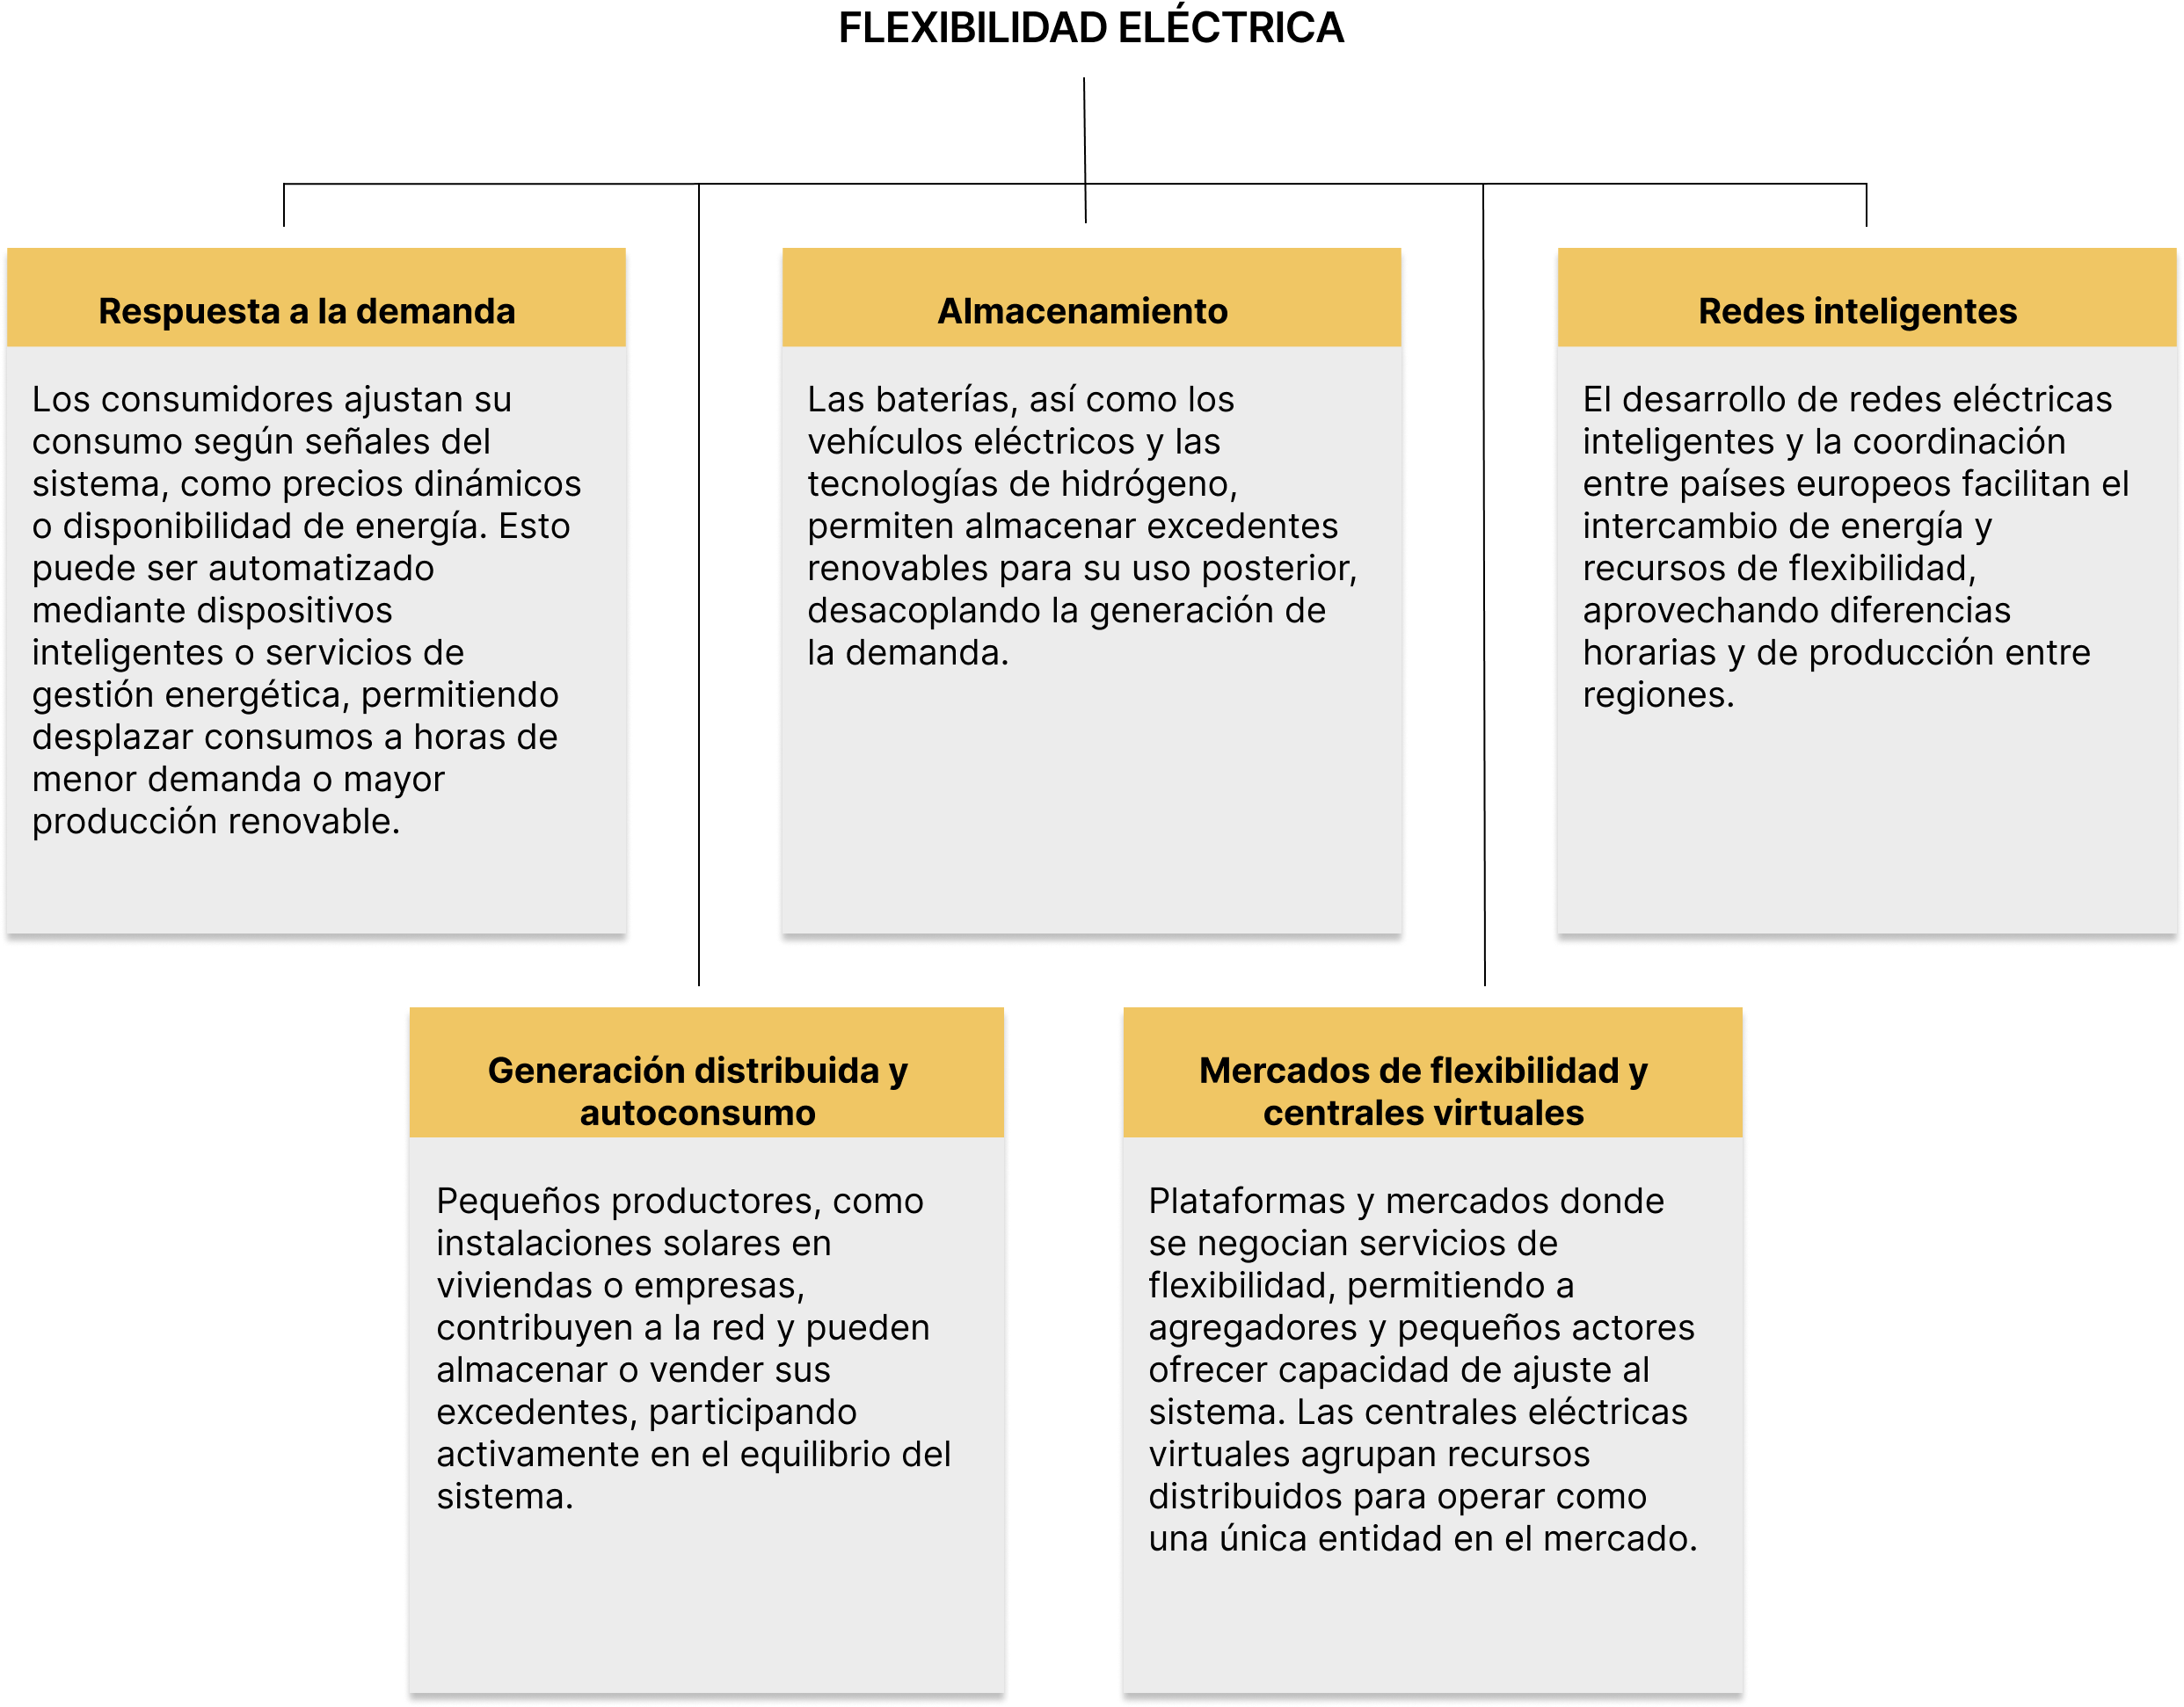
\includegraphics[width=1\linewidth]{fig/image.png}
    \caption{Elementos clave de la flexibilidad eléctrica}
    \label{fig:flexibilidad}
\end{figure}
Como se indicaba anteriormente en este trabajo, la solución aquí \mbox{propuesta} se centra en la flexibilidad del lado de la demanda, por lo tanto cae en el apartado de respuesta a la demanda de este diagrama. En definitiva, nuestra herramienta busca desplazar el consumo de nuestros usuarios a horas de menor demanda o mayor producción renovable, aportando ahorros en el proceso.

\subsection{Modelado, simulación y optimización de sistemas energéticos domésticos}
\label{sec:modelado_simulacion_optimizacion_hems}

La creciente complejidad de los sistemas energéticos domésticos, impulsada por la proliferación de dispositivos inteligentes, la generación distribuida (como paneles fotovoltaicos), el almacenamiento energético (baterías), la carga de \gls{ves} y la exposición a tarifas eléctricas dinámicas, \mbox{exige} herramientas avanzadas para su análisis y gestión eficiente. Los \gls{hems} buscan optimizar el consumo energético en este entorno dinámico, considerando las preferencias del usuario, los costes operativos y las posibles restricciones de la red. Para diseñar y evaluar estrategias de \gls{hems} de manera efectiva, el modelado y la simulación detallados son imprescindibles, permitiendo explorar el comportamiento del sistema bajo diversos escenarios antes de una costosa implementación real.

La \gls{des} emerge como un paradigma particularmente adecuado para modelar la operación de los \gls{hems}. En estos sistemas, los cambios de estado significativos (encendido/apagado de electrodomésticos, inicio/fin de carga del \gls{ve}, cambios en la tarifa eléctrica, eventos de respuesta a la demanda) ocurren en instantes discretos en el tiempo. La literatura ha explorado el uso de \gls{des} para analizar diversos aspectos de la gestión de la demanda residencial, la integración de \gls{ves} y la operación de micro-redes que incluyen componentes domésticos \cite{Lasseter2002, Pipattanasomporn2009}.

Dentro del ámbito de \gls{des}, el formalismo \gls{devs}, propuesto por Zeigler \cite{Zeigler2018}, ofrece un marco matemático riguroso y estructurado para el modelado y \mbox{simulación}. Sus principios de modularidad, jerarquía y encapsulamiento \mbox{facilitan} la construcción de modelos complejos a partir de componentes más simples y \mbox{reutilizables}. Esta capacidad es especialmente valiosa para los \gls{hems}, donde cada dispositivo (lavadora, cargador de \gls{ve}, termostato) puede ser modelado como un componente atómico \gls{devs} con su propia dinámica interna y puertos de interacción, y luego acoplados para representar el sistema doméstico completo. Si bien las aplicaciones de \gls{devs} se han demostrado robustas en dominios como las redes de comunicación y la manufactura \cite{Wainer2013, Liu2008}, y existen trabajos que exploran su uso en el modelado de redes eléctricas y sistemas de potencia \cite{AlHammouri2007, Nutaro2010}, su aplicación específica y detallada para la optimización integrada de \gls{hems} residenciales bajo tarifas dinámicas es un área con un considerable potencial de desarrollo. Este \gls{tfm} adopta el formalismo \gls{devs} para construir un simulador del hogar inteligente que sirva de base para la evaluación precisa de estrategias de gestión de la carga.

Una vez desarrollado un modelo de simulación capaz de replicar el comportamiento energético del hogar, el siguiente desafío es encontrar una política de operación óptima para los dispositivos. Dada la naturaleza combinatoria y a menudo no lineal de los problemas de scheduling de electrodomésticos y cargas en \gls{hems}, especialmente bajo restricciones complejas y tarifas variables, las metaheurísticas se presentan como una solución pragmática y eficiente. Estos algoritmos de optimización, como \gls{sa}, \gls{ag}, o \gls{pso}, son capaces de explorar grandes espacios de búsqueda para encontrar soluciones de alta calidad en tiempos computacionales razonables \cite{Talbi2009}. El algoritmo \gls{sa}, en particular, ha demostrado ser eficaz en problemas de scheduling y optimización combinatoria debido a su capacidad para escapar de óptimos locales \cite{kirkpatrick1983, Logenthiran2012}.

La contribución distintiva de este \gls{tfm} radica en la integración del modelado formal \gls{devs} con un algoritmo de optimización metaheurística (\gls{sa}). En este enfoque, el simulador \gls{devs} no es solo una herramienta de análisis pasivo, sino que actúa como el motor de evaluación (función de \textit{fitness} o coste) dentro del bucle de optimización del \gls{sa}. Cada posible plan de carga generado por el \gls{sa} es simulado detalladamente usando el modelo \gls{devs} del hogar, y el resultado de la simulación (coste energético, picos de demanda, cumplimiento de restricciones) determina la calidad de dicha solución. Esta combinación permite una optimización informada y realista del consumo energético doméstico. A pesar de los avances individuales en simulación \gls{des} y en la aplicación de metaheurísticas a la gestión energética, la literatura específica que documente esta integración de \gls{devs} con \gls{sa} para la optimización de \gls{hems} residenciales multifactoriales es limitada, representando una oportunidad de investigación que este trabajo busca abordar. Por ejemplo, mientras algunos trabajos utilizan \gls{sa} para la gestión de la demanda en redes inteligentes o para la carga de VE \cite{Logenthiran2012, Rajasekhar2021}, la articulación con un modelo de simulación basado en el formalismo \gls{devs} para el hogar completo es menos común.


%-------------------------
\section{Soluciones disponibles en el mercado}
Con el objetivo de entender los productos que ya están disponibles en el mercado, aprender de ellos, e identificar qué servicios de un programa de respuesta a la demanda de carácter residencial son más difíciles de encontrar, comenzamos recogiendo nuestra búsqueda en las siguientes tablas \ref{tab:DERs1}, \ref{tab:DERs2}:

\renewcommand{\arraystretch}{1.3} 

\begin{longtable}{|p{3cm}|p{2cm}|p{5.5cm}|p{1.5cm}|}
    \caption{Algunos programas de respuesta a la demanda residencial en el mercado} \label{tab:DERs1} \\
    \hline
    \textbf{Nombre} & \textbf{Empresa} & \textbf{Breve descripción}\\
    \hline
    \endfirsthead

    \hline
    \textbf{Nombre} & \textbf{Empresa} & \textbf{Breve descripción}\\
    \hline
    \endhead

    \hline Plan de descuento de verano & \cite{Edison2025} & El aire acondicionado central se apaga automáticamente durante los eventos de ahorro.\\
    \hline Programa de Energía Inteligente & \cite{Edison2025} & Un termostato inteligente ajustado automáticamente.\\
    \hline Programa de recompensas de ahorro de energía & \cite{Edison2025} & Reduce el consumo de electricidad durante los eventos entre las 4 p.m. y las 9 p.m., del 1 de mayo al 31 de octubre.\\
    \hline Power Saver Rewards Program & \cite{PG2025} & Reduce el consumo de electricidad durante los eventos entre las 4 p.m. y las 9 p.m., del 1 de mayo al 31 de octubre.\\
    \hline SmartAC™ & \cite{PG2025} & Desvía de forma remota parte del consumo del aire acondicionado fuera de las horas de mayor demanda.\\
    \hline Respuesta de la demanda & \cite{Trane2025} & Adaptan la oferta del DR ajustándolo a las necesidades del cliente, se especializan en aires acondicionados.\\
    
    
    \hline
\end{longtable}

\begin{longtable}{|p{3cm}|p{2cm}|p{5.5cm}|}
    \caption{Algunos programas de gestión activa de dispositivos electrónicos y electrodomésticos en hogares} \label{tab:DERs2} \\
    \hline
    \textbf{Nombre} & \textbf{Empresa} & \textbf{Breve descripción}\\
    \hline
    \endfirsthead

    \hline
    \textbf{Nombre} & \textbf{Empresa} & \textbf{Breve descripción}\\
    \hline
    \endhead

    \hline Google Home + Nest & \cite{Google2025} & Automatiza las tareas y permite monitorizar los dispositivos Google desde cualquier lugar mediante una aplicación o mediante voz.\\
    \hline Alexa Smart Home & \cite{Alexa2025} & Automatiza las tareas y permite monitorizar los dispositivos Amazon desde cualquier lugar mediante una aplicación.\\
    \hline Home Connect & \cite{BSH2025} & Permite controlar los electrodomésticos en una aplicación.\\
    
    
    \hline
\end{longtable}

Esta segunda tabla recoge productos que, aunque no son DR de gestión de la energía al requerir la actuación activa de los usuarios, pueden proporcionar cierta capacidad de adaptación a las tarifas eléctricas variables si se les informa adecuadamente.

Después de realizar esta búsqueda de soluciones y analizar sus prestaciones llegamos a las siguientes conclusiones:
\begin{itemize}
  \item La oferta de DRs se centra en dispositivos concretos, por ejemplo, aires acondicionados, no siendo común la propuesta de un sistema holístico que permita la gestión automática de varios dispositivos diferentes a la vez.
  \item Los servicios más comunes son de carácter estacional, ofreciendo incentivos únicamente durante los meses más calurosos. 
  \item Las grandes empresas tecnológicas han optado por productos que permiten la gestión de productos pertenecientes a sus marcas, necesitando de la intervención del cliente para ello. No se ha identificado ninguna asociación entre estas empresas y otras del sector eléctrico para ofrecer productos que automaticen la gestión de los dispositivos sin la intervención del usuario.
\end{itemize}
En definitiva, están surgiendo productos que buscan aliviar esta problemática y permitir una carga informada de los dispositivos de los usuarios. Además, si bien aún no existen DRs en el mercado público, comienzan a proponerse programas pilotos de diferentes distribuidoras, que comienzan por la gestión de un dispositivo, principalmente los vehículos eléctricos, y después es posible que pivoten a una oferta más holística. Es el caso del plan Inteligent Go de Octopus Energy \cite{octopus2024} o el Asistente Smart Avanzado de Iberdrola \cite{iberdrola2025}. Estas propuestas requieren que el vehículo tenga conectividad y que el usuario indique su hora de salida para que las distribuidoras puedan gestionar las cargas, al igual que la herramienta aquí propuesta. Ambos indican que su sistema de gestión de la carga permite al usuario cargar sus dispositivos en las horas más favorables para los consumidores, no obstante, no se informa de los métodos utilizados para ello. Se sobreentiende el uso de algún tipo de optimización, pero su naturaleza se desconoce. En definitiva, si bien la filosofía de estos productos son similares al propuesto en este \gls{tfm}, falta transparencia sobre el funcionamiento de estos sistemas, y quedan limitados a la carga de vehículos eléctricos. Sin embargo, se espera que programas así evolucionen a ofertas más completas, que permitan la gestión inteligente de una mayor variedad de dispositivos como pretende hacer este proyecto. 

% COMENTARIOS GENERALES

\clearpage
%Metodologia
\chapter{Implementación}
Esta sección detalla el diseño y desarrollo de la solución propuesta, apoyándose en diagramas y fragmentos de código. Se profundiza en la arquitectura del sistema, el funcionamiento de los modelos \gls{devs} implementados y la lógica del algoritmo de optimización para la generación de planes de carga.

%Planificación
\section{Planificación}
Para facilitar el desarrollo de la herramienta se divide esta en cuatro tareas diferentes: recopilación de los datos, desarrollo del simulador, optimización de la simulación y examen de la herramienta, tal como se ilustra en la Figura \ref{fig:plan-desarrollo}.

\begin{figure}
    \centering
    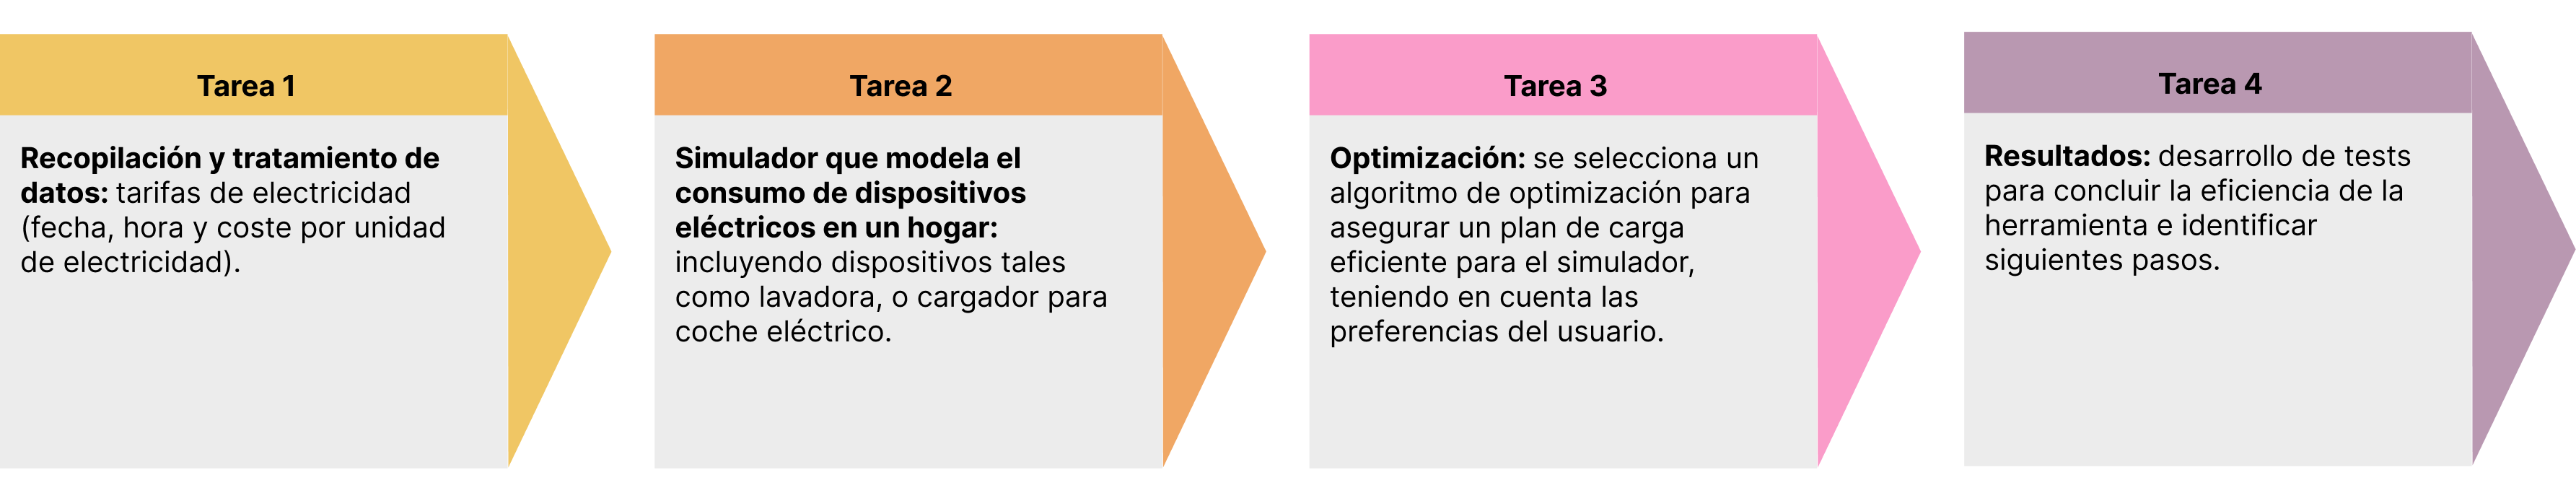
\includegraphics[width=0.95\linewidth]{fig/proceso.png}
    \caption{Plan de desarrollo de la solución}
    \label{fig:plan-desarrollo}
\end{figure}
\section{Diseño}

\subsection{Datos}
Si bien se usan tarifas eléctricas del mercado para la validación robusta en este \gls{tfm}, una aplicación real debería idealmente permitir al usuario introducir su tarifa específica o conectarse a un proveedor de datos de su tarifa. Esto se debe a que el objetivo principal de este tipo de esquemas es dar ahorro al cliente y, en segundo lugar, a la proveedora eléctrica. Además, una tarifa de cliente más baja suele coincidir  con los momentos en los que el precio de mercado también es más asequible. No obstante, al utilizar las tarifas de mercado, que son más dinámicas, conseguimos probar el funcionamiento de esta herramienta para condiciones más complejas. De esta forma garantizamos que nuestra solución sea válida para las nuevas tarifas, que, impulsadas por la flexibilidad de la demanda, tienden a alejarse de los esquemas de tarifa plana para adoptar precios más variables a lo largo del día. 

Al comienzo del código que gestiona el cálculo de los costes y la optimización de ellos se define un array con los valores a utilizar, tal como aparece en el \autoref{lst:tarifas_horarias}.

\begin{lstlisting}[language=Python, caption={Definición de tarifas horarias}, label={lst:tarifas_horarias}]
TARIFAS_HORA = [
    0.07, 0.07, 0.07, 0.07, 0.07, 0.07, #00h-05h (Valle)
    0.13, 0.13, 0.13, 0.13, 0.13, 0.13, #06h-11h (Llano)
    0.19, 0.19, 0.19, #12h-14h (Punta)
    0.13, 0.13, 0.13, #15h-17h (Llano)
    0.19, 0.19, 0.19, 0.19, #18h-21h (Punta)
    0.07, 0.07 #22h-23h (Valle)
]
\end{lstlisting}

Como se expone en el apartado de Objetivos de este trabajo, escogemos una tarifa variable, en este caso con tres franjas horarias diferentes (punta, llana, valle), con el objetivo de otorgar margen para la optimización del consumo, mientras que se dota de suficiente estabilidad a los precios para permitirnos examinar con claridad los resultados de la herramienta.

De manera alternativa, y para dotar a la herramienta de más exactitud, se podría conectar el código con una fuente de datos de tarifas eléctricas reales, si bien, para una primera aproximación al problema esto no resulta necesario.

\subsection{Stack tecnológico}
La solución está programada en Python, utilizando librerías propias de este lenguaje para el desarrollo de las diferentes funcionalidades. Algunas de las librerías utilizadas son:
    \begin{itemize}
    \item xdevs: para la simulación del modelo \gls{devs}.
    \item tkinter y ttkbootstrap: para el desarrollo de la interfaz de usuario.
    \item matplot y numpy para los gráficos de los tests de convergencia.
    \end{itemize}
El código a su vez está publicado en un repositorio en GitHub \cite{ainaralarbi2025}.
\subsection{Arquitectura}
La arquitectura de esta solución incluye tres capas: la capa de presentación, la capa de aplicación y la capa de datos.
La capa de presentación es la que interactúa directamente con los usuarios, ofreciendo una interfaz sencilla de utilizar, mientras que la capa de aplicación gestiona la lógica del sistema. Los scripts de Python operan dentro de esta capa para simular y optimizar las cargas. 
Esta arquitectura se representa de forma simplificada en el diagrama \ref{fig:arquitectura-general}.

\begin{figure}
    \centering
    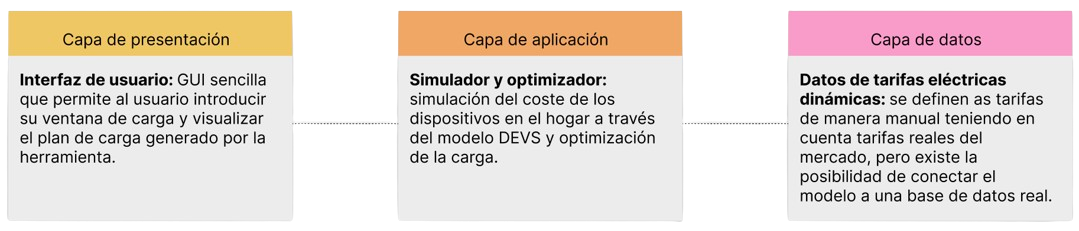
\includegraphics[width=1\linewidth]{fig/Screenshot_2025-04-17_at_20.38.32-removebg-preview.png}
    \caption{Arquitectura general de la herramienta}
    \label{fig:arquitectura-general}
\end{figure}
La arquitectura del sistema se basa en el modelo \gls{devs}, lo que permite representar cada dispositivo del hogar como un sistema autónomo que reacciona a eventos discretos. Cada uno de estos dispositivos está implementado como un modelo atómico, con su propia lógica de estados, duración de funcionamiento y consumo energético.

Estos modelos atómicos están integrados dentro de un modelo acoplado llamado "Casa", que se encarga de conectar los componentes y gestionar el flujo de eventos y energía. La simulación se inicia a partir de un conjunto de eventos, que se emiten desde un componente "Generador". Este generador interpreta eventos en formato hora-dispositivo-acción y los envía al componente correspondiente, activando o desactivando cada aparato.

El sistema cuenta además con un componente "Transducer", que mide métricas clave como el consumo total, el consumo por hora y el pico de energía alcanzado durante la simulación. Estas métricas son fundamentales para evaluar la eficiencia de cada posible plan de carga propuesto.

La lógica de optimización está separada del sistema de simulación. Se hace uso de un algoritmo de tipo \gls{sa} para generar combinaciones de horarios para el uso de los dispositivos, simulando cada combinación con el modelo DEVS completo. Aunque esta aproximación permite una evaluación rigurosa del comportamiento del sistema, puede implicar un elevado coste computacional, especialmente al utilizar algoritmos de tipo poblacional. Por esta razón, y dado que el objetivo principal es minimizar el coste energético total, se opta por emplear el algoritmo \gls{sa}. Esta técnica está especialmente diseñada para explorar de forma eficiente espacios de solución amplios. El algoritmo respeta además las restricciones impuestas por el usuario, como los horarios de disponibilidad del coche y las horas máximas de inicio para los electrodomésticos, usando directamente las duraciones definidas en sus respectivas clases.

Finalmente, se incluye una interfaz gráfica construida con tkinter y ttkbootstrap que permite al usuario introducir sus preferencias de horario y lanzar el optimizador. Esta interfaz presenta el resultado, mostrando el plan de uso elegido y los eventos generados, sin necesidad de interactuar directamente con el código.

\subsection{Interfaz de usuario}
La interfaz de usuario de esta herramienta está basado en las librerías tkinter y ttkbootstrap de Python, y coge la forma de un pop-up. Se trata de una \gls{gui} sencilla que permite al usuario indicar la hora de llegada y la hora de salida y, a partir de estos datos, generar un plan de carga optimizado que se muestra en un calendario. Esta visualización busca mostrar de una manera clara y visual el resultado de la optimización. El calendario se adapta en función de la hora de llegada indicada. La figura \ref{fig:gui} muestra esta interfaz.

\begin{figure}[H]
    \centering
    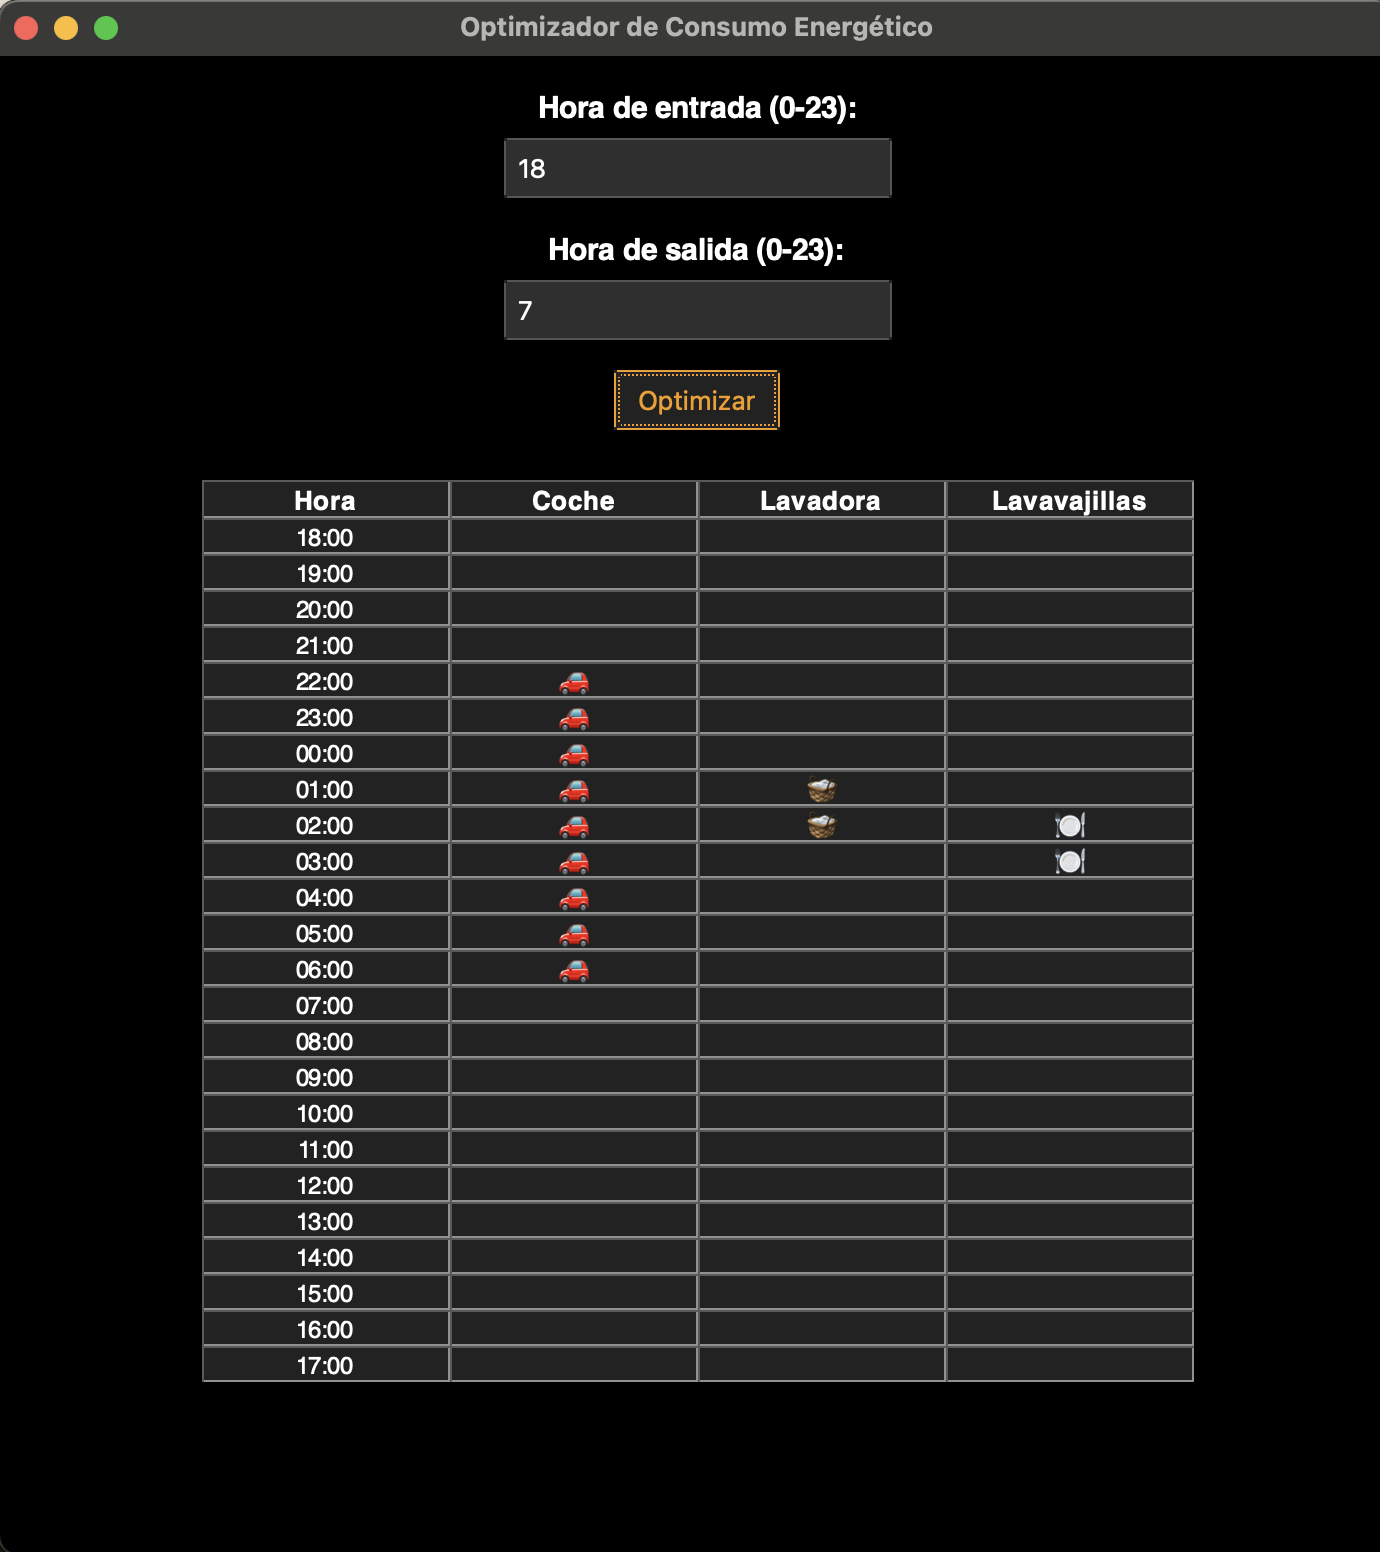
\includegraphics[width=0.75\linewidth]{fig/GUI.png}
    \caption{Interfaz de usuario}
    \label{fig:gui}
\end{figure}
%Funcionamiento
\section{Funcionamiento}

\subsection{Lógica DEVS}
Como se introduce en capítulos anteriores, DEVS es un marco modular y jerárquico utilizado para representar sistemas discretos basados en eventos, lo que nos permite modelar de manera precisa y reutilizable los distintos componentes eléctricos de una casa \cite{fardSimulated2020, Zeigler2018}. A continuación, se explica en más detalle el funcionamiento de los diferentes componentes de nuestro sistema DEVS, con fragmentos de nuestro código para proveer una visión más completa.

% JOSE L: CONTINUAR AQUÍ

\begin{itemize}
    \item \textbf{Modelos atómicos}: Cada dispositivo del sistema (lavadora, lavavajillas, cargador de coche) se implementa como un modelo atómico, compuesto por:
    \begin{itemize}
    \item Funciones de transición interna (deltint)
    \item Funciones de transición externa (deltext)
    \item Función de salida (lambdaf)
    \end{itemize}
    Este modelo representa el ciclo de la lavadora. Recibe una señal de inicio (start) y transiciona por las fases inicio, lavando y passive, calculando la energía consumida durante la fase de lavado, tal como aparece en \autoref{lst:lavavajillas}. El modelo para otros electrodomésticos del estilo se configuran de manera similar.

\begin{lstlisting}[language=Python, caption={Modelo \texttt{Lavavajillas} en DEVS}, label={lst:lavavajillas}]
import logging
from xdevs.models import Atomic, Port
class Lavavajillas(Atomic):
    def __init__(self, name="Lavavajillas", 
    consumo_por_hora: float = 1.2, duracion: float = 1.5):
        super().__init__(name)
        self.duracion: float = duracion
        self.consumo_por_hora: float = consumo_por_hora
        self.i_start = Port(int, "start")
        self.add_in_port(self.i_start)
        self.o_energy = Port(float, "energy")
        self.add_out_port(self.o_energy)
    def initialize(self):
        self.passivate()
    def exit(self):
        pass
    def lambdaf(self):
        if self.phase == "lavando":
            self.o_energy.add(self.consumo_por_hora)
    def deltint(self):
        if self.phase == "inicio":
            self.hold_in("lavando", self.duracion)
        elif self.phase == "lavando":
            self.passivate()
    def deltext(self, e):
        self.continuef(e)
        self.hold_in("inicio", 0.0)
\end{lstlisting}

    \item \textbf{Transductor}: Almacena la energía total, el consumo por hora y los picos de potencia. Funciona acumulando los valores de entrada y registrando las métricas por hora del día. El siguiente fragmento de código, \autoref{lst:transducer},  asegura una medición por hora simulada que permite el cálculo de los costes de las cargas que se necesitan para el optimizador:
    \begin{lstlisting}[language=Python, caption={Método \texttt{deltext} del \texttt{Transducer}}, label={lst:transducer}]
    def deltext(self, e):
    self.continuef(e)
    hora_actual = int(self.clk) % 24  
    self.clk += e
    energia_total_periodo = sum(self.i_energy.values)
    self.energy_t += energia_total_periodo  
    self.energy_consumed += self.energy_t * e
    self.energia_por_hora[hora_actual] += energia_total_periodo
    if self.energy_peak < self.energy_t:
        self.energy_peak = self.energy_t
    self.passivate()
    \end{lstlisting}

    \item \textbf{Modelo acoplado: Casa}: Esta parte del modelo agrupa todos los dispositivos y define cómo se conectan entre sí a través de acoplamientos, incluyendo el generador de eventos y el transductor, tal como aparece en \autoref{lst:casa}.
    \begin{lstlisting}[language=Python, caption={Modelo acoplado \texttt{Casa}}, label={lst:casa}]
class Casa(Coupled):
    def __init__(self, name, file_path=None, events_list=None):
        super().__init__(name)
        if file_path is not None:
            self.generador = Generador("generador", 
            file_path=file_path)
        elif events_list is not None:
            self.generador = Generador("generador", 
            events_list=events_list)
        else:
            raise ValueError("provide events")
        self.lavadora = Lavadora()
        self.lavavajillas = Lavavajillas()
        self.coche = CargadorCoche()
        self.transducer = Transducer()
        self.add_component(self.generador)
        self.add_component(self.lavadora)
        self.add_component(self.lavavajillas)
        self.add_component(self.coche)
        self.add_component(self.transducer)
        self.add_coupling(self.generador.get_out_port("lavadora"), 
        self.lavadora.i_start)
        self.add_coupling(self.generador.get_out_port("lavavajillas"), 
        self.lavavajillas.i_start)
        self.add_coupling(self.generador.get_out_port("coche_start"), 
        self.coche.i_start)
        self.add_coupling(self.generador.get_out_port("coche_stop"), 
        self.coche.i_stop)
        self.add_coupling(self.lavadora.o_energy, 
        self.transducer.i_energy)
        self.add_coupling(self.lavavajillas.o_energy, 
        self.transducer.i_energy)
        self.add_coupling(self.coche.o_energy, 
        self.transducer.i_energy)
\end{lstlisting}
\end{itemize}

\subsection{Algoritmo}
Con el objetivo de encontrar un plan de carga eficiente para los distintos dispositivos de la casa, se ha optado por el algoritmo Simulated Annealing como técnica de optimización. Este algoritmo está inspirado en el proceso físico de enfriamiento de metales y se caracteriza por su capacidad para evitar quedar atrapado en óptimos locales al aceptar peores de forma controlada en las primeras fases de búsqueda \cite{OptimizationSimulatedAnnealing1983}. El resultado de esta optimización es una minimización del coste energético total, teniendo en cuenta las tarifas eléctricas horarias y penalizando los picos de potencia que superen el umbral especificado y las demás restricciones especificadas por el usuario.

Entre las distintas metaheurísticas disponibles, \gls{sa} fue seleccionada frente a otras alternativas como los \gls{ag} por varias razones. En primer lugar, el algoritmo ha demostrado buen rendimiento en problemas de planificación horaria similares al planteado en este trabajo. Por otra parte, a diferencia de los \gls{ag} que requieren mantener y evaluar poblaciones completas de soluciones, \gls{sa} permite trabajar sobre una única solución activa, reduciendo así de manera significativa la carga computacional del sistema. Asimismo, su estructura secuencial facilita la incorporación de restricciones personalizadas del usuario, sin necesidad de diseñar operadores genéticos complejos. Estas características hacen que \gls{sa} hay sido el algoritmo seleccionado para este proyecto. El Algoritmo \ref{alg:sa_general} detalla el funcionamiento de nuestro \gls{sa}.

%pseudo codigo algoritmo
\begin{algorithm}
\caption{Implementación general del algoritmo optimizador Simulated Annealing. Adaptado de \cite{simulatedAnnealingAlgoritmo2021}}
\label{alg:sa_general}
\begin{algorithmic}[1]
\REQUIRE $T_{\text{max}}$ (temperatura inicial), $T_{\text{min}}$ (temperatura mínima), $E_{\text{umbral}}$ (umbral de energía), $\alpha$ (factor de enfriamiento)
\ENSURE Mejor solución encontrada $x$

\STATE $T \leftarrow T_{\text{max}}$
\STATE $x \leftarrow$ generar solución candidata inicial
\STATE $E \leftarrow E(x)$ \COMMENT{calcular energía de la solución inicial}

\WHILE{$T > T_{\text{min}}$ \AND $E > E_{\text{umbral}}$}
    \STATE $x_{\text{nueva}} \leftarrow$ generar nueva solución candidata
    \STATE $E_{\text{nueva}} \leftarrow E(x_{\text{nueva}})$
    \STATE $\Delta E \leftarrow E_{\text{nueva}} - E$

    \IF{Aceptar$(\Delta E, T)$}
        \STATE $x \leftarrow x_{\text{nueva}}$
        \STATE $E \leftarrow E_{\text{nueva}}$
    \ENDIF

    \STATE $T \leftarrow T \cdot \alpha$ \COMMENT{enfriar la temperatura}
\ENDWHILE

\RETURN $x$
\end{algorithmic}
\end{algorithm}

En definitiva:
\begin{enumerate}
    \item Se comienza definiendo una temperatura inicial $T_{\text{max}}$, una temperatura mínima $T_{\text{min}}$, un umbral de energía $E_{\text{umbral}}$ y un factor de enfriamiento $\alpha$. Se genera una primera solución candidata $x$ y se evalúa su energía con la función de coste ($E$).
    
    \item El algoritmo se queda en un bucle mientras se cumpla que $T > T_{\text{min}}$ y $E > E_{\text{umbral}}$ se cumplen. 
    
    \item Se genera una nueva solución "vecina" $x_{\text{nueva}}$, ligeramente diferente de $x$, y se calcula su coste $E_{\text{nueva}}$.
    
    \item Se calcula la diferencia de energía entre vecinos $\Delta E = E_{\text{nueva}} - E$.
    \begin{itemize}
        \item Si la nueva solución es mejor ($\Delta E < 0$), esta se acepta.
        \item Si es peor, se acepta con una probabilidad dependiente de la temperatura: $P = \exp(-\Delta E / T)$. Esto se hace para escapar de mínimos locales en las primeras fases de este proceso.
    \end{itemize}
    
    \item La temperatura se actualiza según $T \leftarrow T \cdot \alpha$, siendo $\alpha$ un factor menor que 1, haciendo así que el sistema se vuelva más restrictivo con el tiempo. Este proceso es lo que llamamos el enfriamiento.
    
    \item El proceso continúa hasta que la temperatura alcanza un valor suficientemente bajo o se cumple el criterio de energía mínima. 
    \item Se devuelve la mejor solución encontrada.
\end{enumerate}

Se ha adaptado este algoritmo a nuestro sistema de la siguiente manera (\autoref{lst:sa}): 
\begin{lstlisting}[language=Python, caption={Algoritmo de Recocido Simulado (\texttt{simulated\_annealing})}, label={lst:sa}]
def simulated_annealing(temp_inicial=1000, temp_final=1, alfa=0.95, 
                        iteraciones_por_temp=20, 
                        hora_conexion=HORA_CONEXION, 
                        hora_objetivo=HORA_OBJETIVO):
    actual = generar_individuo(hora_conexion, hora_objetivo)
    mejor = actual.copy()
    fitness_actual, energia_eur_actual, 
    penalizacion_actual = evaluar_solucion(actual)
    coste_mejor = fitness_actual
    temp = temp_inicial
    while temp > temp_final:
        for _ in range(iteraciones_por_temp):
            vecino = generar_vecino(actual, hora_conexion, hora_objetivo)
            coste_vecino, energia_eur_vecino, 
            penalizacion_vecino = evaluar_solucion(vecino)

            delta = coste_vecino - fitness_actual
            if delta < 0 or random.random() < math.exp(-delta / temp):
                actual = vecino
                fitness_actual = coste_vecino
                energia_eur_actual = energia_eur_vecino
                penalizacion_actual = penalizacion_vecino

                if fitness_actual < coste_mejor:
                    mejor = actual.copy()
                    coste_mejor = fitness_actual
        temp *= alfa
    return mejor
\end{lstlisting}
Para evaluar el \textit{fitness} o la calidad de las soluciones contempladas se define el método evaluar\_solucion(). En esta configuración de la herramienta se tienen varios aspectos en cuenta para evaluar una solución. Estos son los siguientes:
\begin{itemize}
    \item La potencia utilizada no sobrepasa el límite de potencia contratada.
    \item La lavadora y el lavavajillas no comienzan después de una hora establecida. Esto puede ser para evitar el ruido en horas de descanso, o por cualquier otra preferencia del usuario.
    \item Ambos electrodomésticos no funcionan a la vez. Esta penalización no es necesaria, pero muestra cómo el sistema puede adaptarse a los requisitos específicos del hogar mediante nuevas restricciones.
    \item El coche no carga más horas de las estrictamente necesarias.
\end{itemize}
Teniendo en cuenta estas restricciones, se asocian penalizaciones a cada caso y se computa el total para obtener el \textit{fitness} de cada solución. El código utilizado para ello queda recogido en el \autoref{lst:eval}:
\begin{lstlisting}[language=Python, caption={Función \texttt{evaluar\_solucion}}, label={lst:eval}]
def evaluar_solucion(solucion):
    coche_start, coche_stop, hora_lavadora, hora_lavavajillas = solucion
    posibles_horas = horas_validas(HORA_CONEXION, HORA_OBJETIVO)
    if coche_start not in posibles_horas or coche_stop not in 
    posibles_horas:
        return float("inf"), float("inf"), float("inf")
    intervalo = calcular_intervalo_horas(coche_start, coche_stop)
    if intervalo < TIEMPO_CARGA_MINIMO or intervalo > len(posibles_horas):
        return float("inf"), float("inf"), float("inf")
    if not intervalo_dentro_del_rango(coche_start, coche_stop, 
    posibles_horas):
        return float("inf"), float("inf"), float("inf")
    eventos = [
        f"{coche_start};coche_start!1",
        f"{hora_lavadora};lavadora!1",
        f"{hora_lavavajillas};lavavajillas!1",
        f"{coche_stop};coche_stop!1",
    ]
    casa = Casa("casa", events_list=eventos)
    coordinador = Coordinator(casa)
    coordinador.initialize()
    coordinador.simulate(200)
    coordinador.exit()
    transducer = casa.transducer
    energia_por_hora = transducer.energia_por_hora
    energia_peak = transducer.energy_peak
    coste_energia = sum(
        energia * tarifa for energia, tarifa in 
        zip(energia_por_hora, TARIFAS_HORA)
    )
    penalizacion_pico = 0
    if energia_peak > LIMITE_PICO:
        penalizacion_pico = 100000 * (energia_peak - LIMITE_PICO)
    penalizacion_tiempo = 0
    if hora_lavadora + DURACION_LAVADORA > HORA_LIMITE_INICIO:
        penalizacion_tiempo += 1.0
    if hora_lavavajillas + DURACION_LAVAVAJILLAS > HORA_LIMITE_INICIO:
        penalizacion_tiempo += 1.0
    penalizacion_carga_larga = 0
    if intervalo > TIEMPO_CARGA_MINIMO:
        exceso = intervalo - TIEMPO_CARGA_MINIMO
        penalizacion_carga_larga = exceso * 1.0  
    penalizacion_solapamiento = 0
    if hora_lavadora == hora_lavavajillas:
        penalizacion_solapamiento = 1.0
    fitness = coste_energia + penalizacion_pico + 
    penalizacion_tiempo + \
              penalizacion_carga_larga + penalizacion_solapamiento
    penalizacion_total = penalizacion_pico + penalizacion_tiempo + \
                         penalizacion_carga_larga + 
                         penalizacion_solapamiento
    return fitness, coste_energia, penalizacion_total
\end{lstlisting}

En definitiva, esta implementación de un algoritmo \gls{sa} nos permite dar un coeficiente de idoneidad a cada solución contemplada, teniendo en cuenta todas las restricciones indicadas por el usuario.

\chapter{Resultados}
En este capítulo se presentan los resultados de la implementación y evaluación del sistema \gls{hems} propuesto. Se incluyen tanto la validación del algoritmo de optimización como su aplicación en un caso de estudio simulado, con el objetivo de cuantificar los beneficios en términos de ahorro energético.
\section{Test de convergencia}
Una vez definido el funcionamiento de la herramienta propuesta, y desarrollado una \gls{gui} que permite a los usuarios hacer uso de ella, plantemos un test de convergencia que evalúe la eficiencia de nuestra solución.

Este test de convergencia tiene como objetivo analizar cómo evoluciona la calidad de las soluciones obtenidas por el algoritmo propuesto a lo largo de las iteraciones. Este análisis permite observar en qué momento el algoritmo deja de mejorar significativamente sus resultados, identificando así un posible punto de saturación en la búsqueda \cite{keepcoding2023convergencia}. Para ello, se monitoriza la evolución del mejor valor de la función de \textit{fitness} encontrado por el algoritmo en cada iteración. Se ejecutan varias simulaciones, en este caso cinco, con el objetivo de evaluar la estabilidad y velocidad de convergencia del algoritmo, facilitando la elección de un número de iteraciones adecuado que optimice el equilibrio entre precisión y tiempo de cómputo. 

Para la configuración del test, se hace uso de un escenario base para un hogar equipado con varios dispositivos programables, un perfil de conexión entre las 18:00 y las 23:00, y tarifas energéticas que distinguen entre periodos valle, llano y punta cómo las presentadas anteriormente. Las restricciones también son las indicadas en secciones anteriores. Se utiliza la librería matplot para visualizar la gráfica resultante. 

El código utilizado es el presentado en \autoref{lst:test}:

\begin{lstlisting}[language=Python, caption={Convergencia del algoritmo de Recocido Simulado}, label={lst:test}]
def simulated_annealing_tracking(temp_inicial=1000, temp_final=1, 
alfa=0.95, iteraciones_por_temp=20, hora_conexion=HORA_CONEXION, 
hora_objetivo=HORA_OBJETIVO):
    actual = generar_individuo(hora_conexion, hora_objetivo)
    mejor = actual.copy()
    fitness_actual, _, _ = evaluar_solucion(actual)
    fitness_mejor = fitness_actual
    temp = temp_inicial
    historico_mejores = []
    while temp > temp_final:
        for _ in range(iteraciones_por_temp):
            vecino = generar_vecino(actual, hora_conexion, hora_objetivo)
            fitness_vecino, _, _ = evaluar_solucion(vecino)
            delta = fitness_vecino - fitness_actual
            if delta < 0 or random.random() < math.exp(-delta / temp):
                actual = vecino
                fitness_actual = fitness_vecino
                if fitness_actual < fitness_mejor:
                    mejor = actual.copy()
                    fitness_mejor = fitness_actual
            historico_mejores.append(fitness_mejor)
        temp *= alfa
    return historico_mejores
\end{lstlisting}

La gráfica resultante queda recogida en la Figura \ref{fig:convergencia}.

\begin{figure}[H]
    \centering
    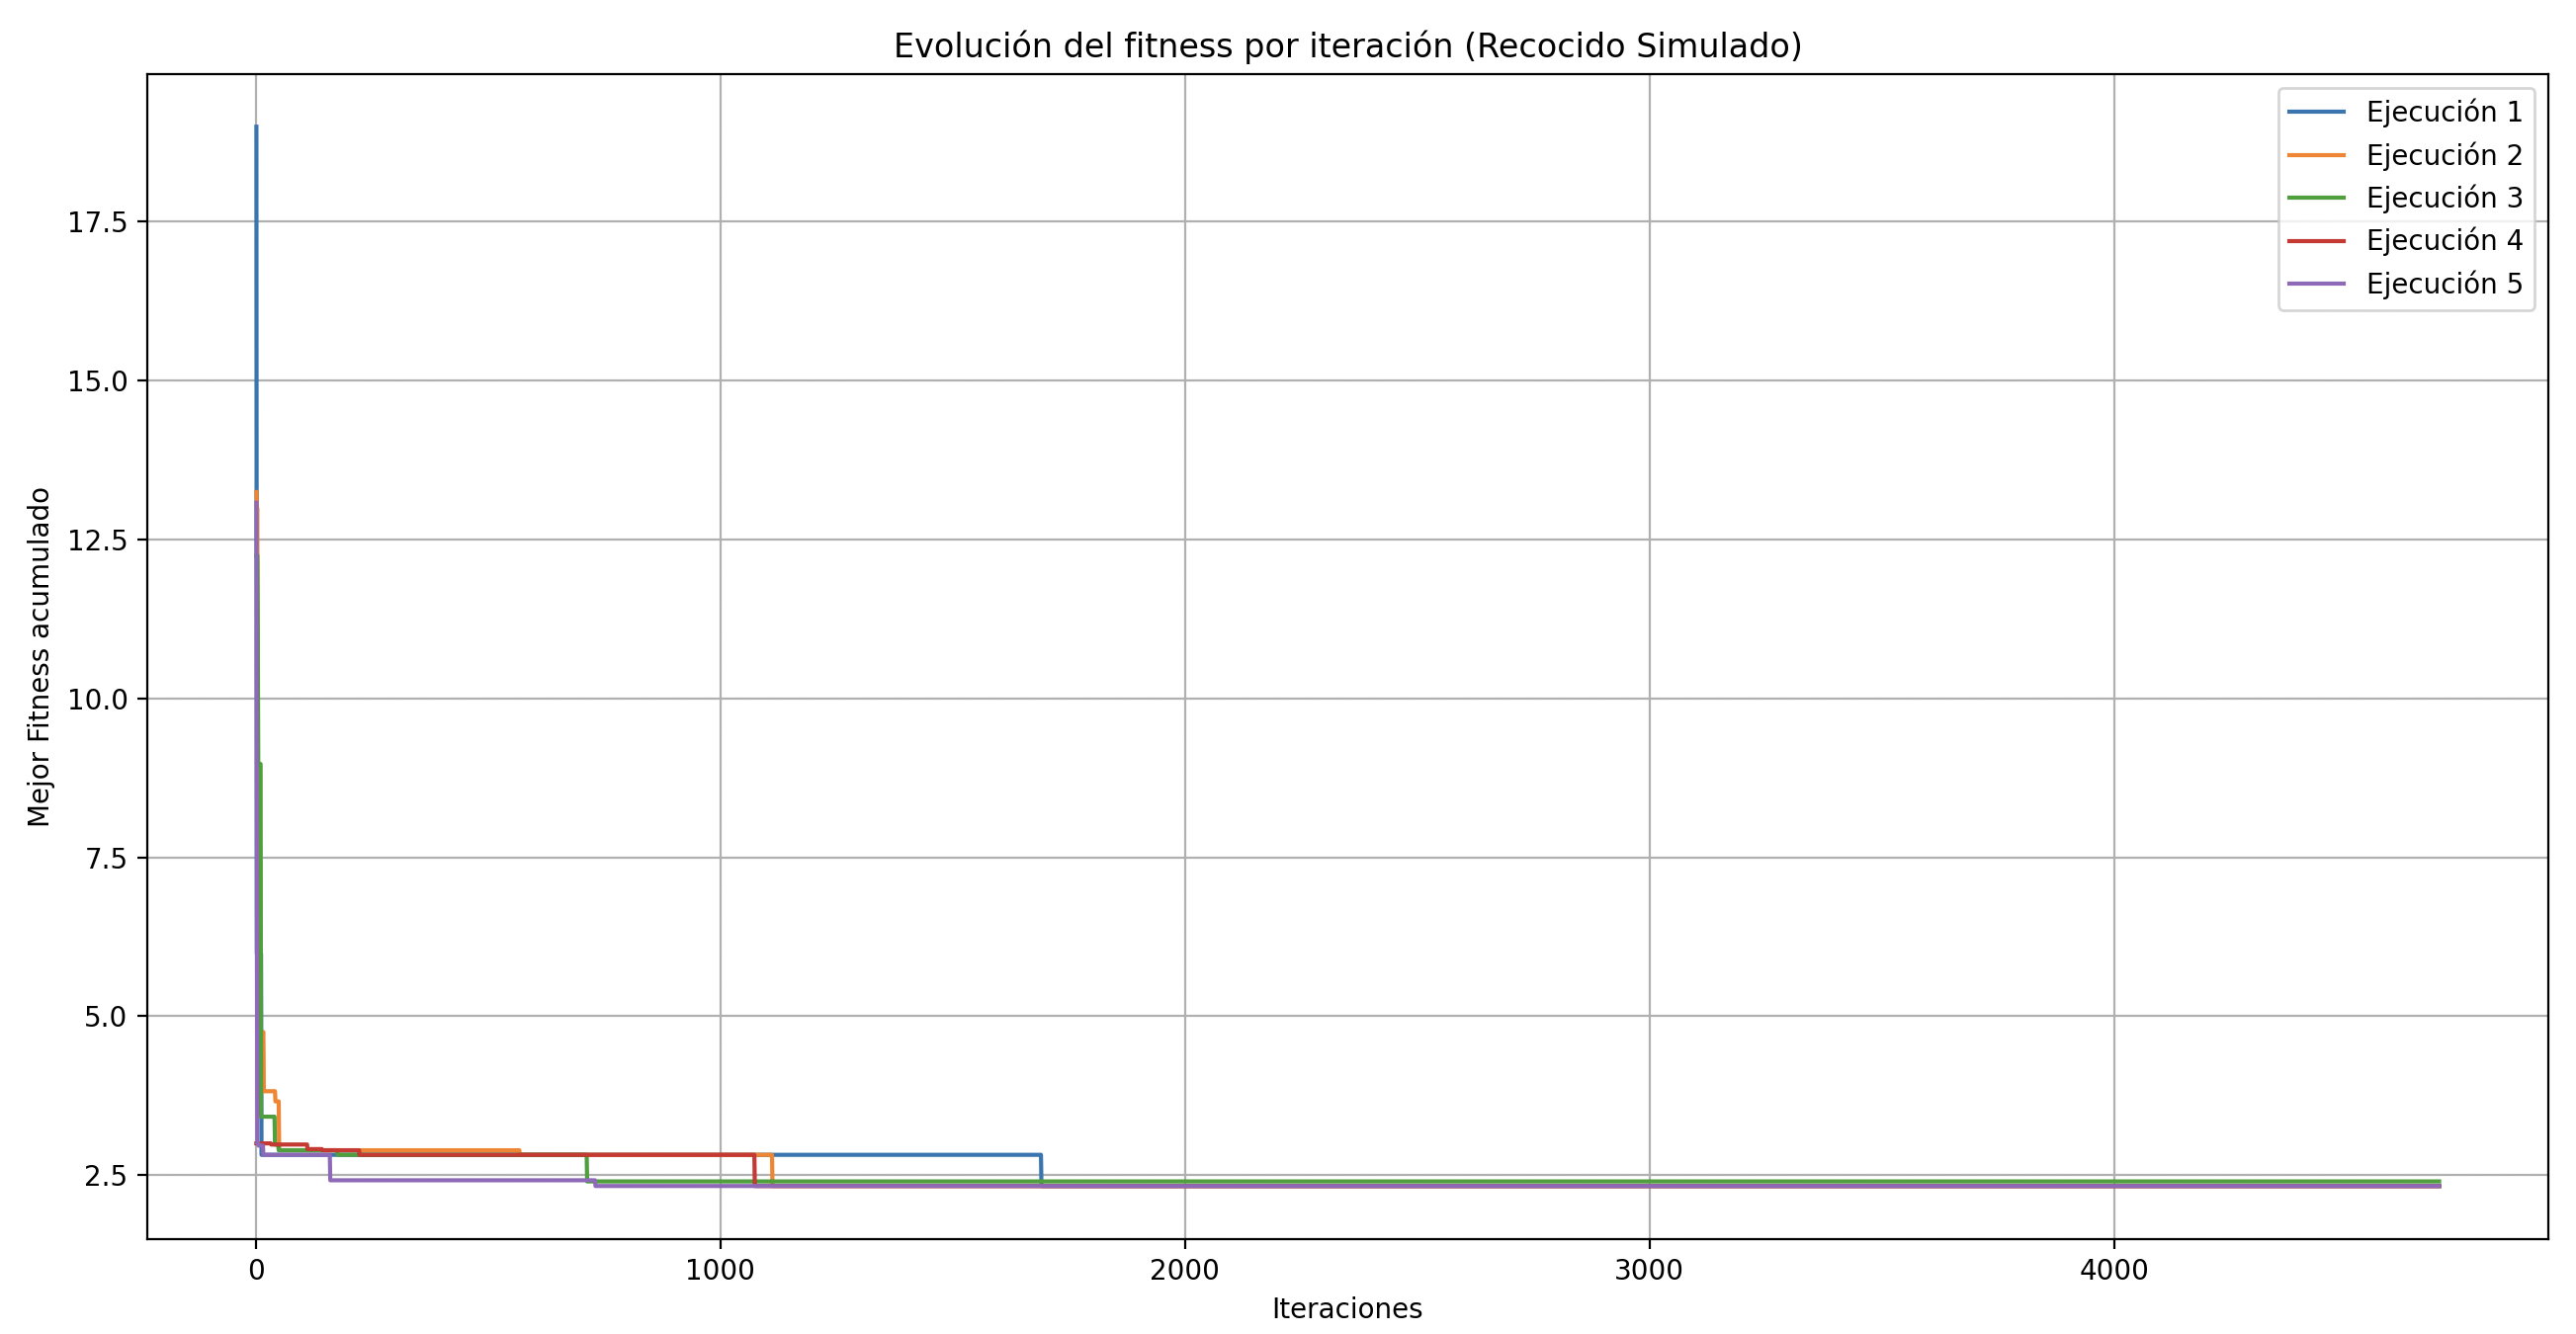
\includegraphics[width=1.1\linewidth]{fig/convergencia.png}
    \caption{Evolución del mejor valor de fitness por iteración}
    \label{fig:convergencia}
\end{figure}

En la figura se muestra la evolución del mejor valor de la función de \textit{fitness} alcanzado por el algoritmo \gls{sa} a lo largo de las iteraciones, en cinco ejecuciones independientes. Se observa que en las primeras iteraciones, especialmente antes de las 500 primeras, se produce una rápida disminución del \textit{fitness}, lo que indica que el algoritmo encuentra soluciones significativamente mejores en las fases iniciales del proceso. A partir de ese punto, las mejoras son cada vez más esporádicas, tendiendo a estabilizarse hacia valores cercanos a 2.5 en todas las ejecuciones. Este valor corresponde a una métrica combinada de coste energético total y penalizaciones por incumplimiento de restricciones. Esta convergencia temprana sugiere que, a partir de 1500 iteraciones, el algoritmo muestra una tendencia a estabilizarse, aportando mejoras marginales que podrían no justificar el coste computacional adicional.

Este análisis resulta útil para optimizar el tiempo de ejecución del algoritmo, ya que permite identificar un número de iteraciones suficiente para obtener soluciones de buena calidad sin generar costes computacionales innecesarios. Por lo tanto, se concluye que para nuestra herramienta un límite de 1500-2700 iteraciones es adecuado para garantizar una convergencia eficiente del algoritmo.

A partir de este test se concluyen los parámetros de la tabla \ref{tab:parametros_sa} como los más adecuados para la solución propuesta:
\renewcommand{\arraystretch}{1.2}

\begin{longtable}{>{\raggedright\arraybackslash}p{4.5cm} c >{\raggedright\arraybackslash}p{8cm}}
    \caption{Parámetros utilizados en la implementación del algoritmo SA}%
    \label{tab:parametros_sa} \\
    \toprule
    \textbf{Parámetro} & \textbf{Valor} & \textbf{Descripción} \\
    \midrule
    Temperatura inicial \( T_0 \) & 1000 & Valor inicial alto que permite explorar el espacio de soluciones sin restricciones iniciales. \\
    Temperatura final \( T_{\text{final}} \) & 1 & Umbral que determina la condición de parada del proceso de enfriamiento. \\
    Factor de enfriamiento \( \alpha \) & 0.95 & Factor multiplicativo para reducir la temperatura en cada ciclo. \\
    Iteraciones por temperatura & 20 & Número de soluciones generadas por cada valor fijo de temperatura. \\
    Iteraciones totales (aprox.) & 2700 & Derivado del número de ciclos necesarios para alcanzar \( T_{\text{final}} \) desde \( T_0 \), con el esquema de enfriamiento definido.\footnotemark \\
    \bottomrule
\end{longtable}

\footnotetext{
Dado que la temperatura se actualiza como \( T_{k+1} = \alpha \cdot T_k \), se necesitan aproximadamente 135 ciclos para que \( T < T_{\text{final}} \) con \( T_0 = 1000 \), \( T_{\text{final}} = 1 \) y \( \alpha = 0.95 \). Esto implica un total aproximado de \( 135 \times 20 = 2700 \) iteraciones.
}

Además de la validación técnica del algoritmo propuesto y sus resultados en términos de convergencia, cabe destacar la relevancia práctica de esta herramienta para los usuarios.

\section{Estudio de caso: ahorro generado por el uso de la herramienta \gls{hems}}
Con el objetivo de evaluar el impacto práctico de la herramienta desarrollada, se plantea una comparativa entre el precio que supondría para el usuario cargar todos sus dispositivos a la hora de entrada a la casa, frente al coste generado si el usuario siguiera el plan de carga presentado por la herramienta. Para este análisis no se tienen en cuenta restricciones ni penalizaciones para el cálculo del escenario sin optimización.

\begin{itemize}
    \item \textbf{Escenario sin optimización:} todos los dispositivos comienzan su funcionamiento a las 18:00.

    \begin{itemize}
        \item Coche eléctrico: 18:00–21:00 \(\rightarrow\) tarifa: 0{,}19~\euro{}/kWh
        \item Lavadora: 18:00–20:00 \(\rightarrow\) tarifa: 0{,}19~\euro{}/kWh
        \item Lavavajillas: 18:00–19:30 \(\rightarrow\) tarifa: 0{,}19~\euro{}/kWh
    \end{itemize}
    \noindent Coste total estimado: 1{,}79~\euro{}
    \item \textbf{Escenario con optimización:} se emplea \gls{sa} para determinar un plan de carga más beneficioso.
    \begin{itemize}
        \item Coche eléctrico: 22:00–01:00 \(\rightarrow\) tarifa: 0{,}07~\euro{}/kWh
        \item Lavadora: 20:00–22:00 \(\rightarrow\) tarifa: 0{,}13~\euro{}/kWh
        \item Lavavajillas: 22:00–23:30 \(\rightarrow\) tarifa: 0{,}07~\euro{}/kWh
    \end{itemize}
    \noindent Coste total estimado: 0{,}71~\euro{}
\end{itemize}
Para el planteamiento de estos escenarios se han tenido en cuenta la duración de encendido de cada dispositivo. Se ha utilizado las 18h, ya que es una hora Los costes energéticos diarios estimados en ambos escenarios se presentan en la Tabla \ref{tab:estudio_caso_coste}.

\begin{table}[H]
    \centering
    \caption{Comparativa del coste energético diario con y sin optimización}
    \label{tab:estudio_caso_coste}
    \begin{tabular}{lcc}
        \toprule
        \textbf{Escenario} & \textbf{Coste estimado (\euro{})} & \textbf{Ahorro (\%)} \\
        \midrule
        Sin optimización      & 1.79 & -- \\
        Con optimización (SA) & 0.71 & 60.3 \\
        \bottomrule
    \end{tabular}
\end{table}

Es decir, el uso de la herramienta propuesta permite reducir el coste diario de 1.79\euro{} a 0.71\euro{}, representando un ahorro aproximado del 60\%. Esto se da como consecuencia del desplazamiento del consumo eléctrico hacia franjas horarias con tarifas más económicas. Cabe destacar que el ahorro sería mayor si se tuviera en cuenta el impacto de penalizaciones asociadas a restricciones como no utilizar los electrodomésticos a la vez. 

En definitiva, utilizando el sistema propuesto no sólo se contribuye a la distribución de la demanda de consumo eléctrico, aliviando así la presión de la red eléctrica, sino que también supone un ahorro directo para el usuario.
%Conclusiones
\chapter{Conclusiones y trabajo futuro}
La utilidad de esta herramienta se manifiesta en varios niveles. A nivel individual, permite al usuario reducir sus costes energéticos mediante una gestión automatizada que se adapta a tarifas dinámicas, y evita picos de consumo y otras restricciones penalizadas. A nivel colectivo, contribuye a una demanda más distribuida, evitando sobrecargas en la red eléctrica y fomentando el consumo en horas valle, lo que beneficia tanto a los operadores del sistema como al conjunto del sistema energético.

Desde el punto de vista de las ciudades conectadas o inteligentes, esta herramienta representa un componente clave dentro de una infraestructura energética más amplia. Su integración con dispositivos IoT, medidores inteligentes y plataformas de gestión energética permite la creación de hogares que interactúan dinámicamente con la red, ajustando su consumo en función del contexto tarifario, de señales de demanda o incluso de previsiones meteorológicas \mbox{asociadas} a la producción renovable.

En un paso futuro, este tipo de soluciones podrán formar parte de sistemas de respuesta activa a la demanda, agregación de consumos domésticos para mercados energéticos locales y micro redes, o coordinación con comunidades energéticas. En decir, el aporte no se limita a la optimización local de un hogar, sino que se vela por una visión más global de sostenibilidad y autonomía energética.

En definitiva, la herramienta desarrollada cumple los objetivos identificados tras explorar los trabajos y soluciones disponibles en esta área de trabajo. Se logra la implementación de un optimizador de consumo energético doméstico basado en técnicas de simulación \gls{devs} y algoritmos de búsqueda \gls{sa}. Para ello, se \mbox{modela} el comportamiento de dispositivos eléctricos (cargador de coche, lavadora y lavavajillas) y se desarrolla una optimización que considera tanto el coste energético como penalizaciones varias. Además, se proponen análisis de convergencia para ajustar los parámetros del algoritmo, mejorando así su eficiencia y realizando una validación técnica de la solución. 

Los resultados obtenidos permiten a los usuarios lograr un uso energético más eficiente, permitiendo así la generación de ahorro tanto para estos como para las distribuidoras energéticas, además de facilitar una distribución más óptima del consumo eléctrico. En definitiva, este proyecto no solo ha cumplido con los objetivos propuestos, sino que también establece una base sólida para futuras ampliaciones y ofertas más completas.

\subsection{Limitaciones}
Cabe indicar que la eficiencia de esta herramienta viene condicionada por la capacidad de conectividad de los dispositivos del usuario. Es decir, para poder ejecutar el plan de carga propuesto por esta herramienta es necesario la \mbox{existencia} de una panel de control a los que los dispositivos a gestionar estén conectados, y que permita su control en remoto. Esto se trata de un condicionante muy limitante, que si bien se verá disminuido por la alta penetración en el mercado de dispositivos inteligentes conectados, a fecha actual resulta una barrera de adopción importante. Sin embargo, en los casos en los que esta gestión a distancia de los dispositivos no sea posible, esta herramienta puede servir como un sistema de recomendaciones que el usuario puede decidir utilizar para así sacar los beneficios de esta carga más económica.

Por otra parte, la implementación actual está limitada a un hogar específico, sin embargo, si la solución se expendiese a un núcleo energético mayor, como una comunidad energética, sería necesario escalar de manera acorde la capacidad computacional de la solución. Esto es puesto que cada iteración del optimizador requiere de una simulación completa del comportamiento energético del sistema, lo que implica una mayor complejidad y tiempo de cómputo a medida que se incrementa el número de dispositivos y de restricciones a considerar. En ese contexto, podrían explorarse estrategias de paralelización, o el uso de técnicas de evaluación aproximada para mantener tiempos de respuesta razonables sin comprometer la calidad de las soluciones.

\subsection{Trabajo futuro}
La interfaz de usuario aquí planteada es bastante sencilla puesto que los objetivos de este trabajo buscaban desarrollar un primer diseño que permita al usuario interactuar con la herramienta, pero si se quisiera dotar de más sofisticación a la interfaz se proponen los mock-ups de la figura \ref{fig:mock-up}.
\begin{figure}
    \centering
    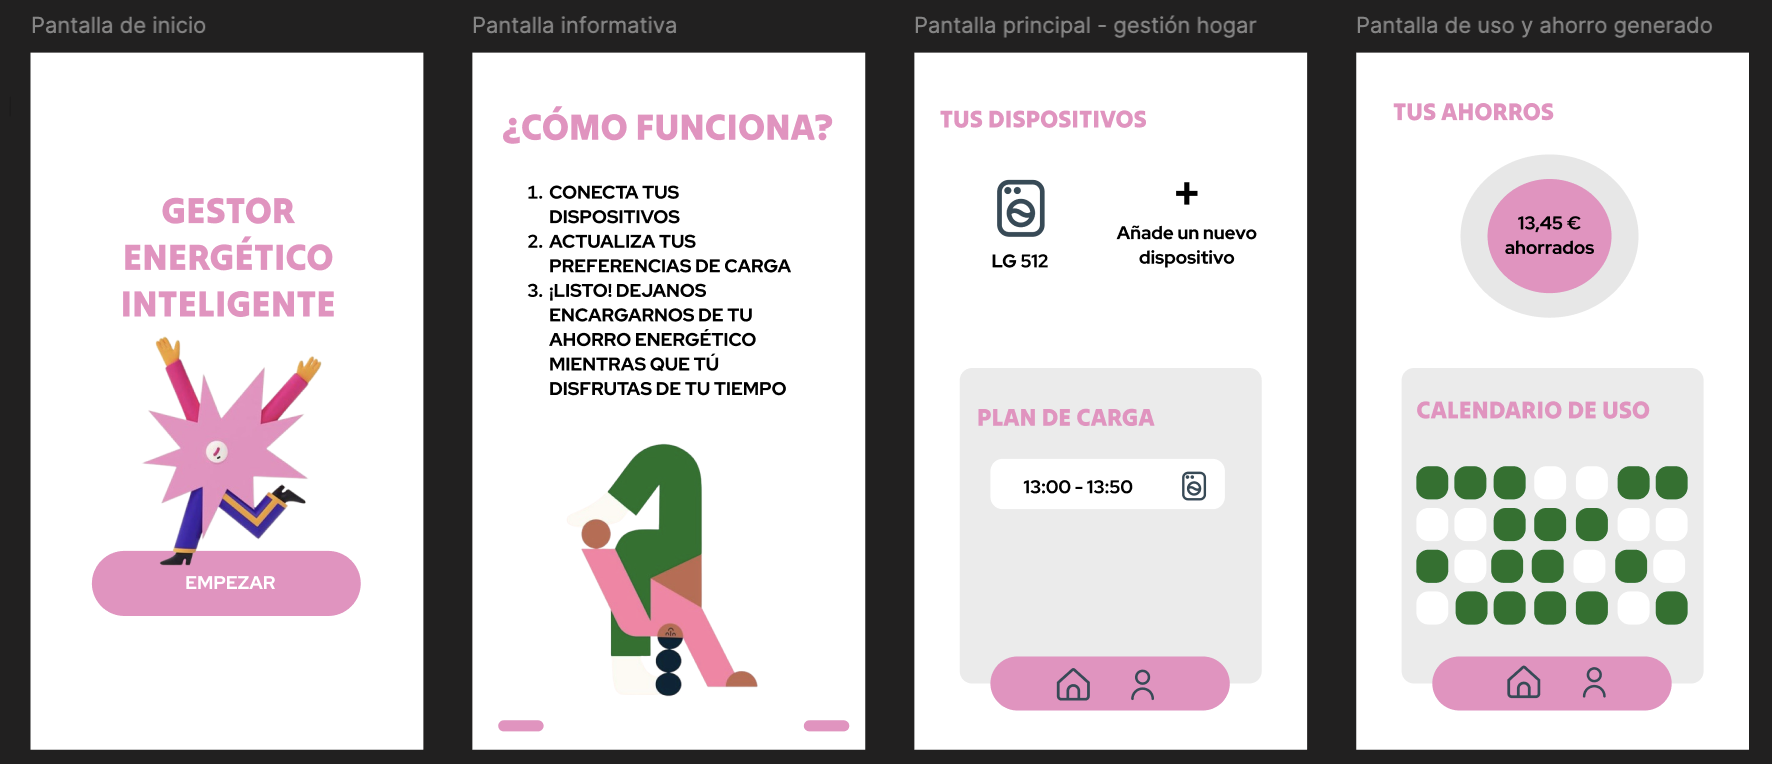
\includegraphics[width=0.95\linewidth]{fig/mockups.png}
    \caption{Mock-ups interfaz de usuario}
    \label{fig:mock-up}
\end{figure}
En esta propuesta de interfaz, el usuario cuenta con dos pantallas principales a las que gana acceso una vez ha pasado por las dos primeras páginas de bienvenida. La primera recoge todos los dispositivos del usuario, permitiendo vincular nuevos. Para que estos se puedan añadir a nuestro gestor de energía inteligente es necesario que los dispositivos estén previamente conectados con el panel de control central de la casa, para asegurar que estos sean controlables de manera remota y que seamos capaces de recolectar datos de los mismos. En la parte baja de la pantalla se encuentra el plan de carga formulado según las preferencias del usuario, para que el cliente esté informado de los detalles de carga de sus electrodomésticos y/o vehículos. En la segunda pantalla, el usuario puede ver sus ahorros generados en el último mes, que se calcularían simulando el coste de la carga de los dispositivos en las horas picos frente al coste real generado, y, además, incluye un calendario de uso de la herramienta para que entienda mejor la relación de su uso con el ahorro generado.

Por otra parte, al no contar con datos en tiempo real, el usuario debe indicar manualmente el tiempo de llegada del vehículo. No obstante, una vez que esta herramienta esté conectada a un panel de control de hogar que tenga conexión directa a los coches vinculados, esto no será necesario. Se propone entonces esta funcionalidad para una versión conectada de esta herramienta.

Finalmente, como se ha mencionado en secciones anteriores de este trabajo, la escalabilidad de esta herramienta está diseñada para que este sistema se aplique a contextos energéticos más amplios, dando cobertura a redes de hogares más extensas y pudiendo albergar un mayor número de restricciones. Queda, por tanto, abierta la posibilidad de implementar esta solución a integraciones más complejas. 

%Bibliografia
\bibliographystyle{IEEEtran}
\bibliography{biblio}

\end{document}
